\setchapterimage[7cm]{at2019fdr/AT2019fdr.jpg}
\chapter{Candidate TDE \emph{AT2019fdr}: A Possible Source?}\label{at2019fdr}
\labch{AT2019fdr}
\emph{AT2019fdr}\marginnote{Light from the candidate TDE \textit{AT2019fdr} illuminating the surrounding dust in an artistic impression. Image credit: DESY and Science Communication Lab.} emerged as a candidate when following up the high-energy IceCube neutrino \emph{IC200530A}. The gold alert\sidenote{See Section~\ref{ic_event_selection}} neutrino was detected on May 30, 2020 with a \SI{90}{\percent} rectangular uncertainty area of \SI{25.4}{\square\deg}, a signalness of 0.59 and an estimated neutrino energy of \SI{82.2}{\tera\eV}~\cite{IC200530A1}.

Two more sources were initially published by us as candidate sources (\textit{SN2020lls} and \textit{SN2020lam}), but both could be ruled out with follow-up observations. For details on these events, see Section~\ref{SN2020lls} and~\ref{SN2020lam}. This left \emph{AT2019fdr} as the only remaining neutrino source candidate, a long-lived optical transient located at RA $= 257.278575$ and Dec $= +26.855758$, with a distance of \SI{1.72}{\degree} to the reported neutrino best-fit location.

At the moment of neutrino arrival, the transient was already 400 days old. It was originally discovered May 13, 2019 by \texttt{AMPEL}~\sidecite{at2019fdr_disc}, with a first detection on May 3, 2019. The neutrino arrived about 10 months after the optical peak. The peak flux in the ZTF \textit{g}-band was \SI{1.3e-12}{\erg\per\s\per\square\cm}. The redshift of $z=0.2666$ was inferred from the Balmer lines visible in a spectrum taken on July 3, 2019 with the Double Spectrograph (DBSP) on the P200 telescope. The peak \textit{g}-band luminosity calculated with this redshift, $L_\text{peak}=\SI{2.9e44}{\erg\per\s}$, showed that \emph{AT2019fdr} was an extraordinarily luminous event\sidenote{Here and in the following sections a standard flat cosmology will be used, with $\Omega_\Lambda = 0.7$ and $H_0=\SI{70}{\km\per\s\per\mega\parsec}$.}.

The long-duration flare was initially tentatively classified as a superluminous supernova of type IIn (SLSN IIn). A peculiarity of this event is that it occured close to the core of its host galaxy SDSSCGB 6856.2, a Narrow-Line Seyfert 1 (NLSy1) galaxy, a type of AGN (see Section~\ref{agn}). The mean angular separation to the host position as reported in the \textit{Gaia} DR2 was \num{0.03 \pm0.15} arcsec. Due to this proximity, it was systematically followed up by a ZTF program dedicated to study flares in NLSy1 galaxies~\sidecite{Frederick2021}.

In a paper describing the sample of such flares detected during ZTF Phase I, a TDE interpretation of \emph{AT2019fdr} was stipulated~\cite{Frederick2021}. The authors outright rejected a SLSN interpretation, and also argued against an AGN origin of the flare. The reasons for disfavoring the SLSN hypothesis were the long-lived \textit{U}-band and UV emission, emission at the blue end of the Balmer line profiles, the longevity of the flare and its nuclear location close to the center of its host galaxy~\cite{Frederick2021}.

\begin{figure*}[htb]
    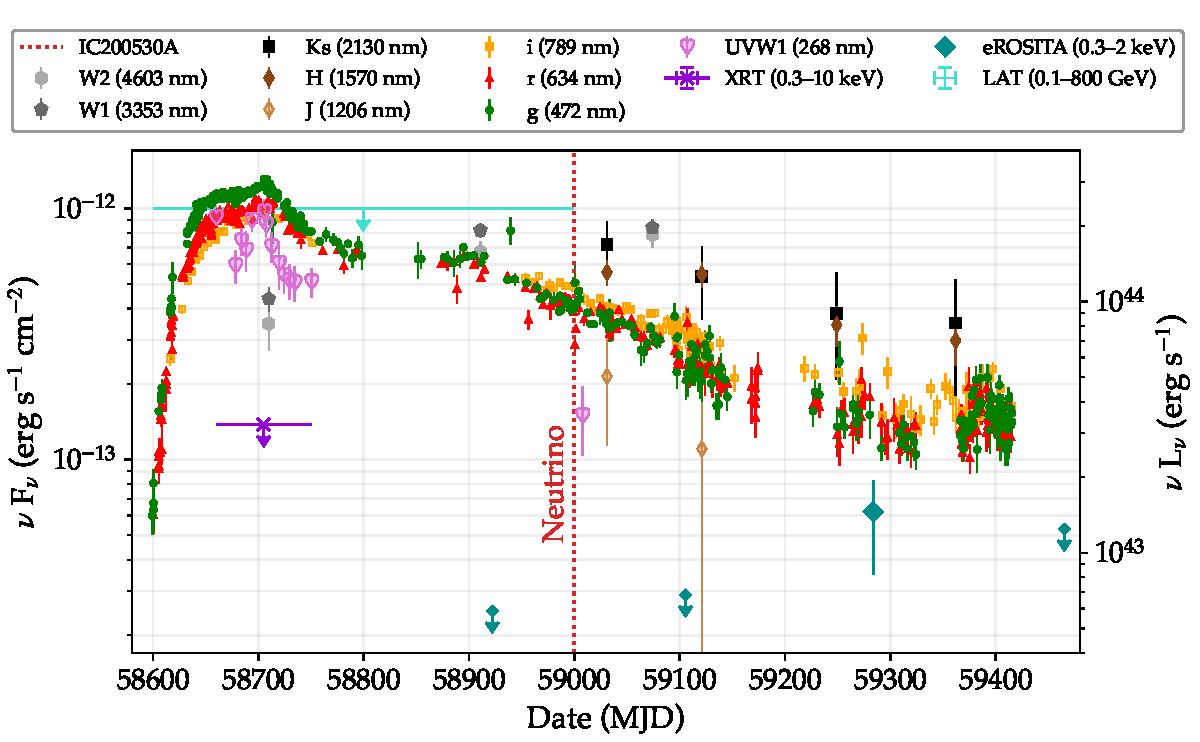
\includegraphics{at2019fdr/at2019fdr_light_curve_flux.pdf}
    \caption[\emph{AT2019fdr} light curve]{Light curve of \emph{AT2019fdr}. The arrival time of \emph{IC200530A} is marked with a red dotted line. It comprises host-subtracted measurements from \textit{WISE}, P200/WIRC, ZTF and \textit{Swift}/UVOT. Also shown are measurements without host subtraction from \textit{SRG}/eROSITA, as well as upper limits from \textit{Swift}/XRT and \textit{Fermi}/LAT. The left y-axis shows $\nu F_\nu$, where $F_\nu$ is the spectral flux density at frequency $\nu$; the right y-axis shows $\nu L_\nu$ with $L_\nu$ being the luminosity at frequency $\nu$. Figure by the author, from~\cite{Reusch2022}.}
    \labfig{at2019fdr_light_curve}
\end{figure*}

In the following, an overview will be given over the observations in different wavelengths, the reductions of the near infrared observations triggered by our group, the modeling of the spectral energy distribution (SED), and the interpretation of the delayed infrared signal as dust echo. This will be followed by a discussion of the TDE interpretation and the calculation of the chance of observing an event comparable to \emph{AT2019fdr} in temporal and spatial coincidence with a high-energy neutrino.

Due to its multi-messenger nature and the large number of instruments involved, the study of \textit{AT2019fdr} was a collaborative effort. Therefore, I have highlighted computing work, reductions or analyses that were done by me personally by explicitly writing `I'. When I was only involved in the discussion and interpretation of results, I wrote `we'.

\section{Multi-wavelength Observations}
As \emph{AT2019fdr} was discovered close to the core of its host galaxy, it was followed up as part of regular ZTF TDE group activities from early on, including ToO observations by \textit{Swift} UVOT and XRT.

After observing the neutrino, I triggered additional follow up with \textit{Swift}/UVOT and requested multi-epoch near-infrared observations with the Wide Field Infrared Camera (WIRC)~\sidecite{Wilson2003} on the P200. Furthermore, our group triggered multi-epoch radio observations with VLA.

Additionally, we analyzed data by the LAT~\cite{Atwood2009} aboard the \textit{Fermi Gamma-Ray Space Telescope} (\textit{Fermi}), and investigated four epochs of observations by the Extended Roentgen Survey with an Imaging Telescope Array (eROSITA) telescope~\sidecite{Predehl2021} aboard the \textit{Spectrum Roentgen Gamma} (\textit{SRG})~\sidecite{Sunyaev2021} space mission.

All detections and upper limits except for the radio data are shown in Fig.~\ref{fig:at2019fdr_light_curve}. As one can see, the flare was very long-lived, with a moderately fast rise (\SI{\sim100}{\day} until optical peak), a short decay phase followed by a plateau, and lastly an exponential decay, apparently with a constant decay rate~\sidecite{Reusch2022}.

\subsection{Gamma-ray Limits}

\begin{marginfigure}
    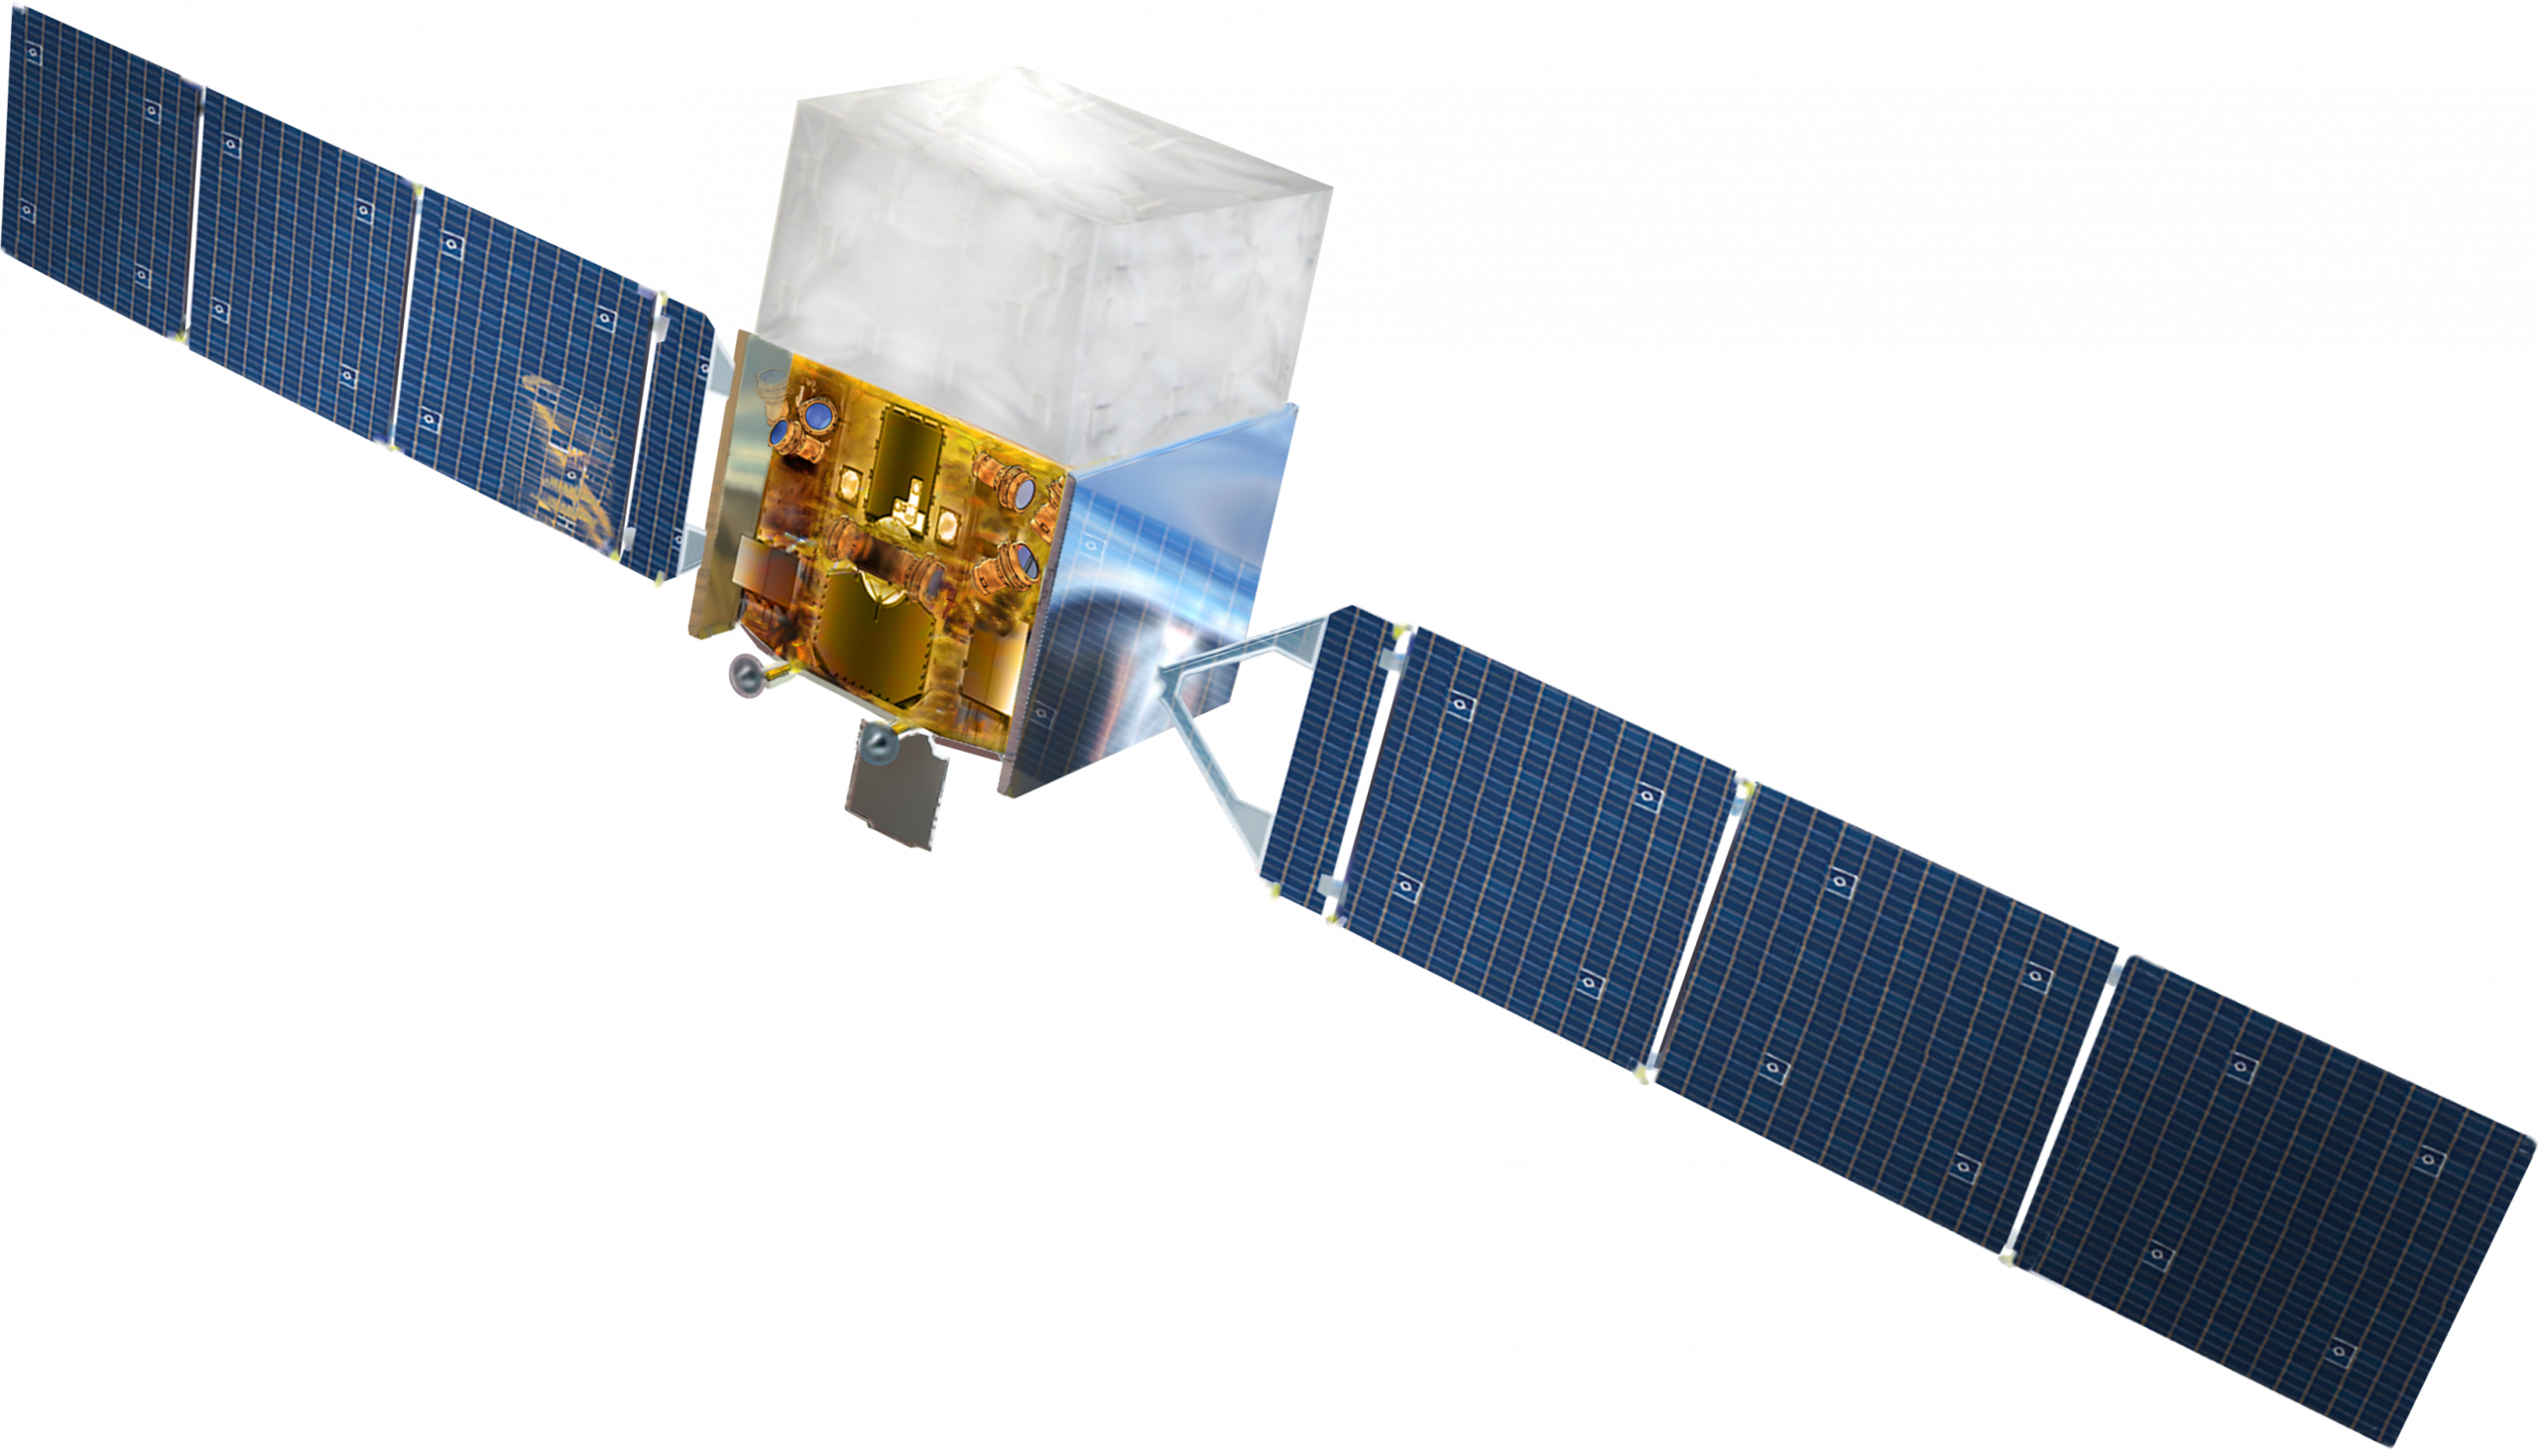
\includegraphics{at2019fdr/fermi.png}
    \caption[The \textit{Fermi} satellite]{The \textit{Fermi} satellite. Image credit: NASA.}
    \labfig{fermi_satellite}
\end{marginfigure}

The details of the \textit{Fermi}/LAT analysis were published in~\sidecite{Velzen2021}. The one year time window analyzed for \emph{AT2019fdr} spanned from the first optical detection of the source on May 3, 2019, until the arrival of the neutrino on May 30, 2020.

No gamma-ray sources were detected significantly (\SI{\geq5}{\sigma}), neither new sources nor previously known sources from the 10 year \textit{Fermi} LAT Fourth Source Catalog (4FGL-DR2)~\sidecite{Abdollahi2020,Ballet2020}. The \SI{95}{\percent} confidence level (CL) upper limit derived for this timeframe within the energy bin of \SIrange{0.1}{800}{\giga\eV} was \SI{1e-12}{\erg\per\s\per\square\cm}. This upper limit was calculated by testing a point-source hypothesis at the location of \emph{AT2019fdr}, assuming a power-law spectrum of the form $\text{d}N/\text{d}E \propto E^{-\gamma}$, with a spectral index $\gamma=2$~\cite{Velzen2021}.

\subsection{X-ray Observations}\label{x_ray_obs}

\begin{marginfigure}
    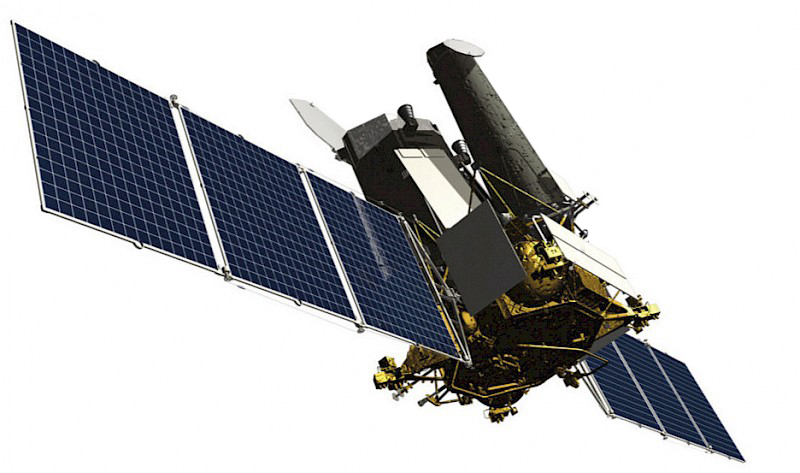
\includegraphics{at2019fdr/SRG.jpeg}
    \caption[The \textit{SRG} satellite]{The \textit{SRG} satellite. The eROSITA instrument aboard \textit{SRG} was put into hibernation following the Russian invasion of Ukraine in February 2022. Image credit: Roskosmos.}
    \labfig{srg_satellite}
\end{marginfigure}

The sky region of AT2019 was visited four times by \textit{SRG} with a six-month cadence. The first visit was March 13--14, 2020. Only on the third visit one year later the source was detected, which can be counted as evidence for temporal evolution in X-ray wavelengths. All measurements and the upper limits and detections derived from these are displayed in Fig.~\ref{fig:at2019fdr_light_curve} and listed in Table~\ref{tab:at2019fdr_erosita}.

\begin{table}
    \begin{center}
        \begin{tabular}{c c c c}
            \hline
            \textbf{MJD} & \textbf{Date} & \textbf{Upper limit}              & \textbf{Energy flux}                                         \\
                         &               & (\unit{\erg\per\s\per\square\cm}) & (\unit{\erg\per\s\per\square\cm})                            \\
            \hline
            \hline
            58922        & 2020--03--14  & \num{2.5e-14}                     & ---                                                          \\
            59105        & 2020--09--13  & \num{2.9e-14}                     & ---                                                          \\
            59284        & 2021--03--11  & ---                               & \num[parse-numbers = false]{6.2^{+2.7}_{-2.1}\times10^{-14}} \\
            59465        & 2021--09--08  & \num{5.3e-14}                     & ---                                                          \\
            \hline
        \end{tabular}
    \end{center}
    \caption[\emph{AT2019fdr} \textit{SRG}/eROSITA detections \& upper limits]{\textit{SRG}/eROSITA upper limits and detection of \emph{AT2019fdr} in the \SIrange{0.3}{2.0}{\kilo\eV}-band. From~\cite{Reusch2022}.}\label{tab:at2019fdr_erosita}
\end{table}

The single detection from March 11, 2021 revealed a very soft thermal spectrum. As can be seen in Fig.~\ref{fig:erosita_fit}, the best-fit blackbody temperature was \SI[parse-numbers = false]{56^{+32}_{-26}}{\eV}, with the errors being \SI{68}{\percent} for one parameter of interest~\sidecite[7pt]{Sazonov2021}. In the source rest frame, this measurement corresponds to a temperature of \SI[parse-numbers = false]{71^{+41}_{-33}}{\eV}. This renders the X-ray spectrum of \emph{AT2019fdr} one of the softest spectra of the TDEs discovered by \textit{SRG}/eROSITA so far.

The equivalent neutral hydrogen column density had a best-fit value of $\text{NH}=\SI[parse-numbers = false]{1.47^{+2.80}_{-1.25}\times10^{21}}{\per\square\cm}$. This value is a measure of the amount of neutral hydrogen atoms along the line of sight to the source. Within the errors it was consistent with the galactic value of $\text{NH}_\text{Gal} = \SI{0.40e21}{\per\square\cm}$. There was some degeneracy between the neutral hydrogen column density and the inferred blackbody temperature; this is usual for soft sources. However, with $T_\text{bb}=\SI{131}{\eV}$ at the \SI{95}{\percent} confidence level, the temperature upper bound was still fairly low~\cite{Reusch2022}.

\begin{figure}[htb]
    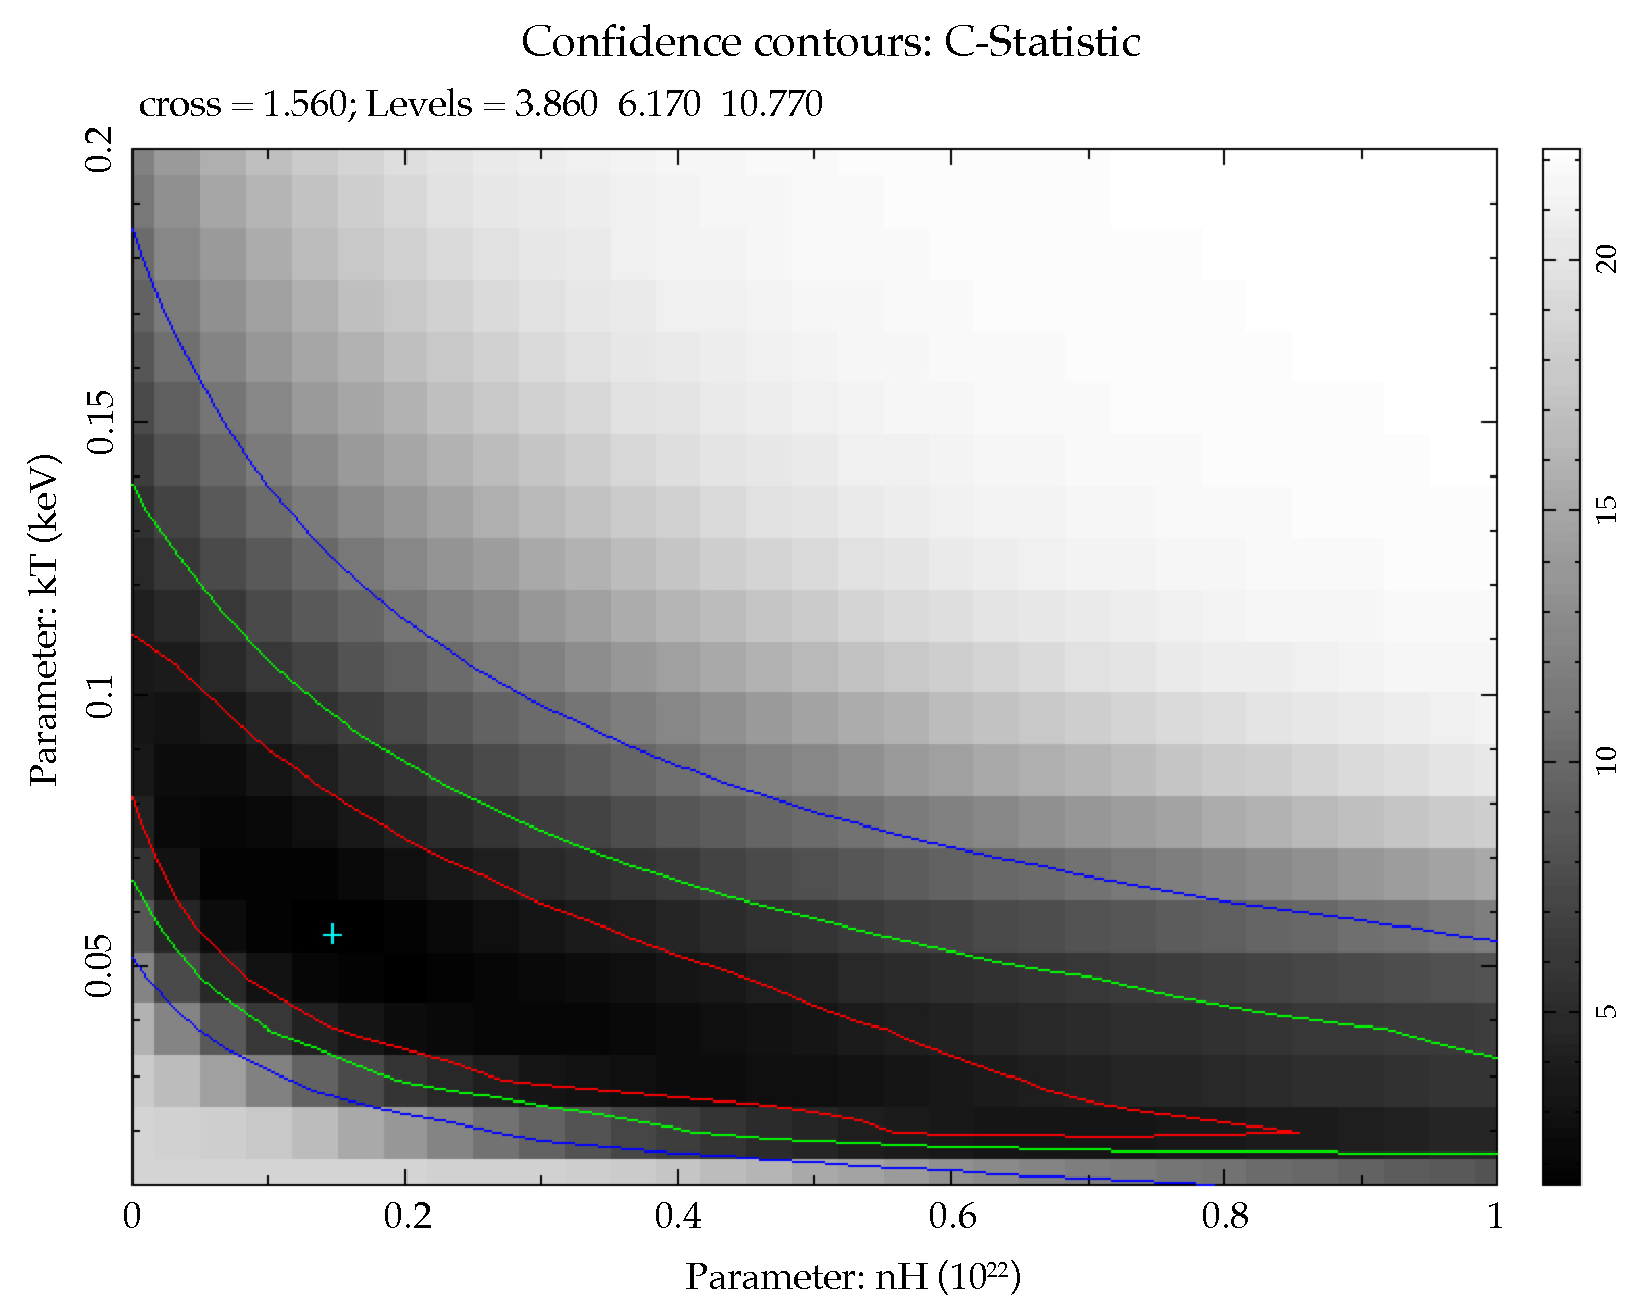
\includegraphics[width=0.8\textwidth]{at2019fdr/erosita_fit.pdf}
    \caption[\textit{SRG}/eROSITA temperature fit]{Temperature fit for the \textit{SRG}/eROSITA detection. Figure by M. Gilfanov, slight modifications by the author.}
    \labfig{erosita_fit}
\end{figure}

As noted above, \textit{Swift} XRT had already observed \emph{AT2019fdr} 14 times prior to the neutrino arrival~\cite{Frederick2021}. We requested a prompt ToO observation after the source emerged as a neutrino candidate, which was carried out on June 7, 2020 with a \SI{2000}{\s} exposure.

The data was reduced with the publicly available \texttt{\textit{Swift} XRT data products generator}~\sidecite{Centre2020} in the energy range of \SIrange{0.3}{10}{\kilo\eV}. As all 14 observations prior to the neutrino arrival were non-detections, those were binned (total exposure: \SI{20700}{\s}) to compute a \SI{3}{\sigma} energy flux upper limit of \SI{1.4e-13}{\erg\per\s\per\square\cm}. The upper flux limit for the post-neutrino observation was \SI{4.7e-12}{\erg\per\s\per\square\cm}. To convert photon counts to to energy flux, I employed the \texttt{HEASARC WebPIMMS} tool~\sidecite{Arida2020}. I set the blackbody temperature to the \SI{56}{\eV} measured by \textit{SRG}/eROSITA, and used the best-fit neutral hydrogen column density from the same measurement~\cite{Reusch2022}.

\begin{marginfigure}
    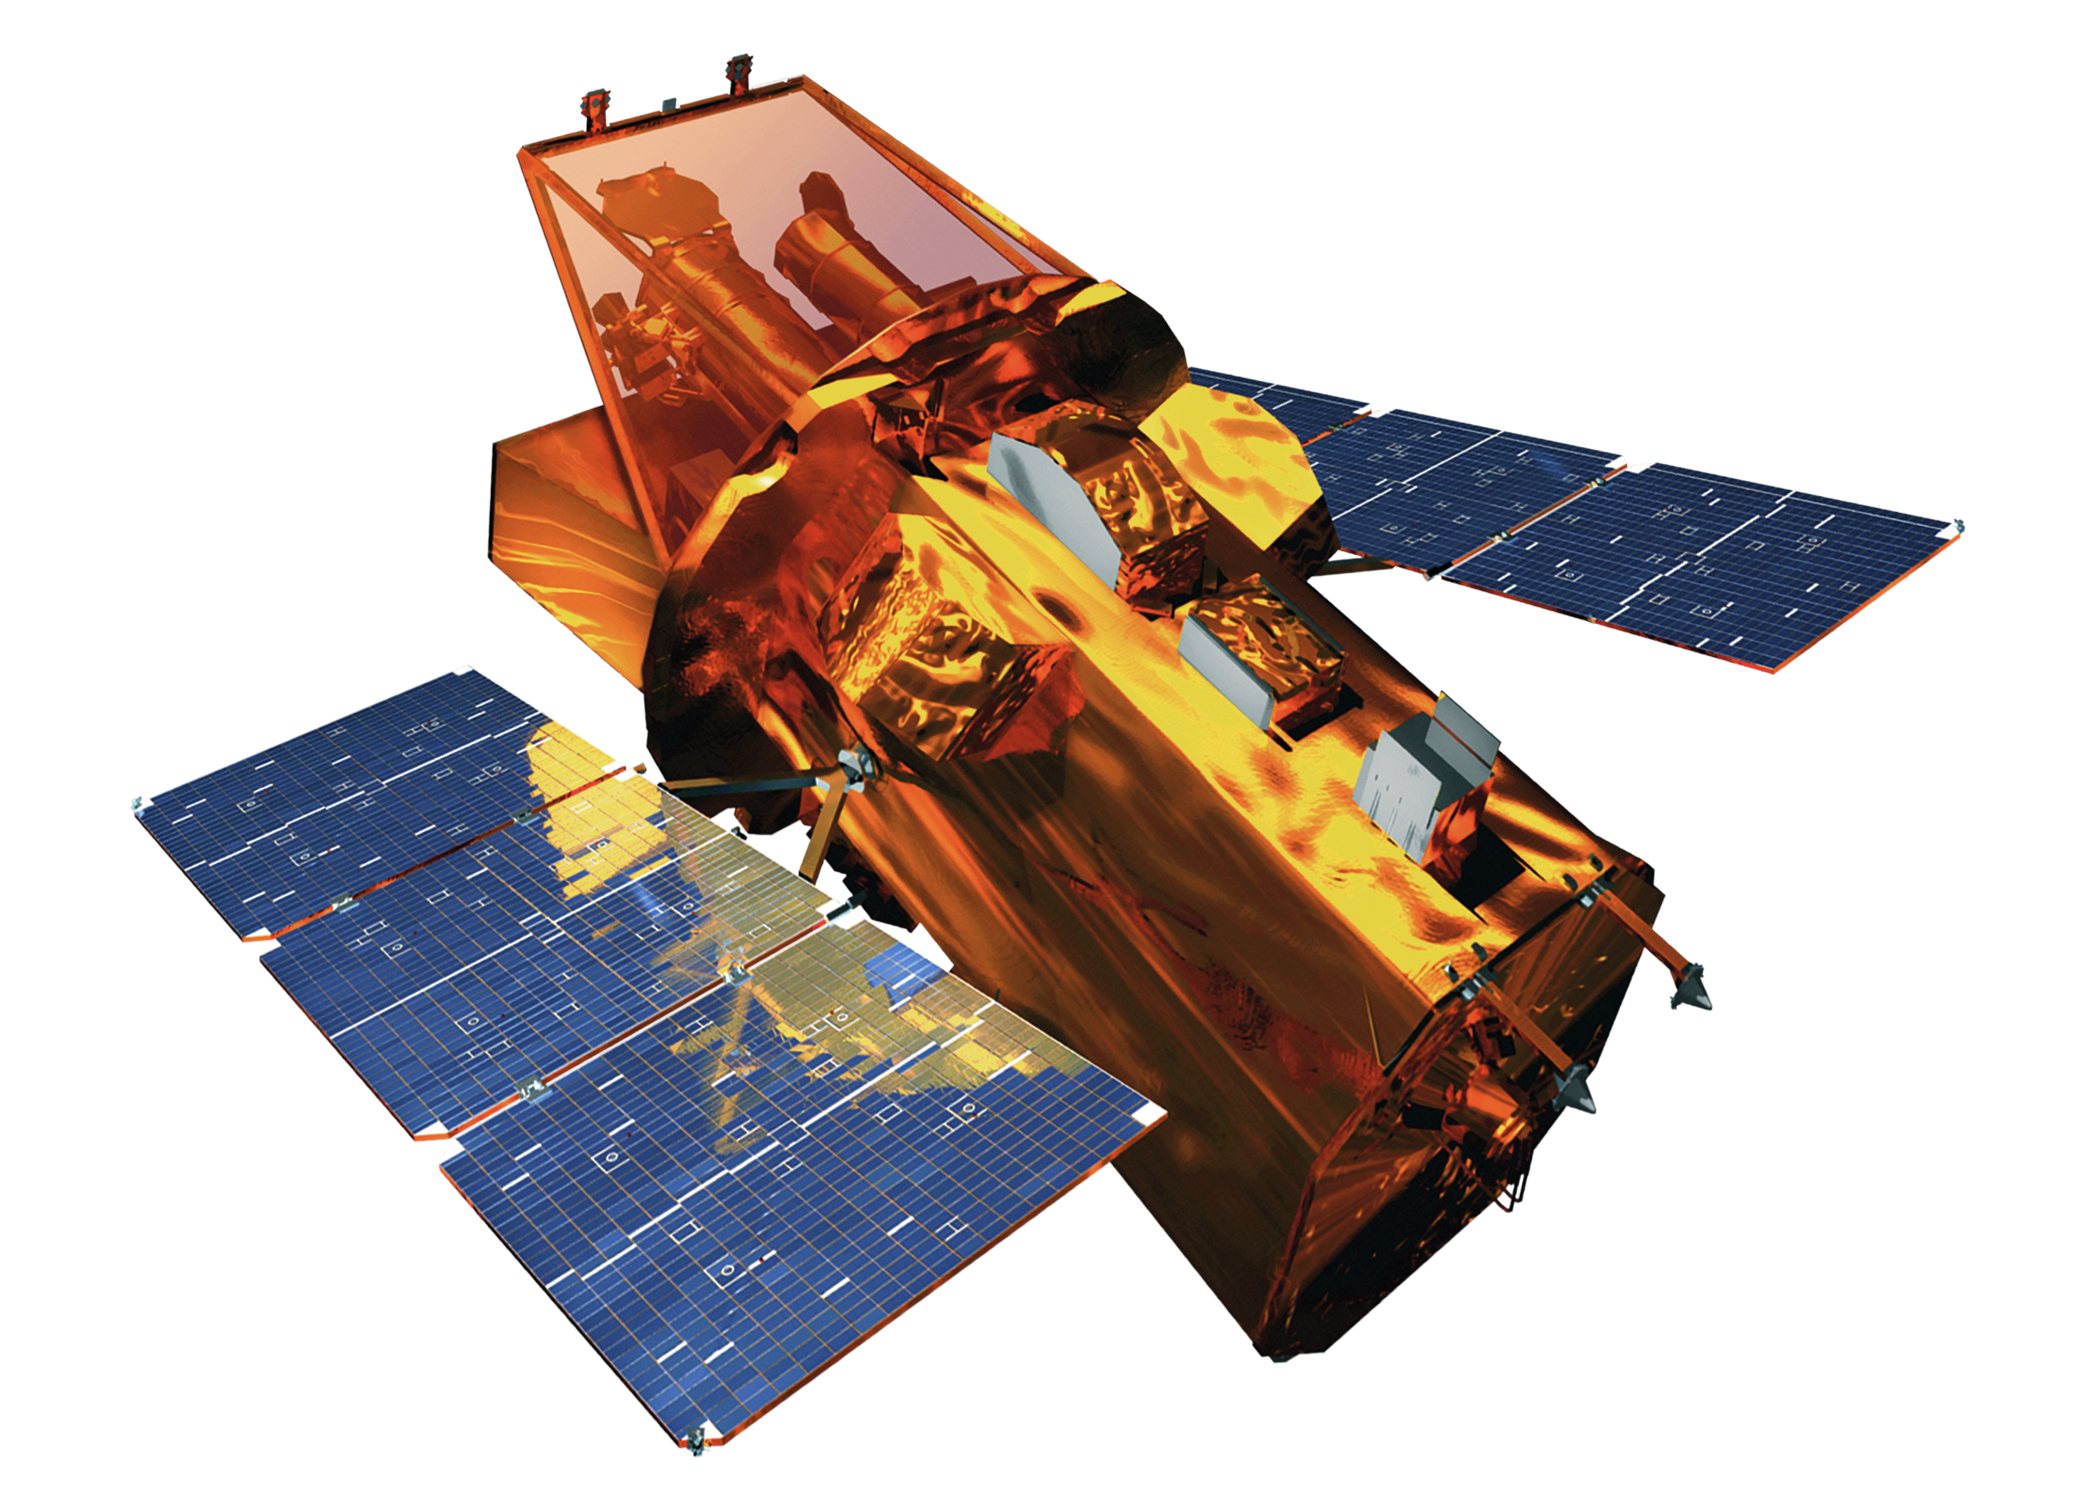
\includegraphics{at2019fdr/swift.png}
    \caption[The \textit{Swift} satellite]{The \textit{Swift} satellite. Image credit: NASA.}
    \labfig{swift_satellite}
\end{marginfigure}

\subsection{Optical/UV Observations}
I processed the ZTF optical observations with \texttt{fpbot} (see Section~\ref{fpbot}). The science-ready \textit{Swift} data was retrieved from the \textit{Swift} archive\sidenote{\url{https://www.swift.ac.uk/swift_portal}}. All exposures of individual epochs were co-added, and filtered to boost the signal-to-noise ratio with \texttt{uvotsim}, contained in \texttt{HEAsoft}\sidenote{\url{https://heasarc.gsfc.nasa.gov/docs/software/heasoft}}. The brightness of the transient was measured using \texttt{uvotsource} of the same package. The aperture used was \num{3} arcsec, with a far bigger radius used for the background level extraction. We calibrated the photometry with files made available by September 2020 and employed the methods of~\sidecite{Breeveld2011} to convert the measured magnitudes to the AB system (see Section~\ref{magnitudes}). I corrected the extracted and converted magnitudes by subtracting the synthetic host model described in Section~\ref{synthetic_host_model}~\cite{Reusch2022}.

As the extraction of the infrared measurements was more involved due to the presence of host galaxy blending, this will be detailed in Section~\ref{nir_reductions} below.

\subsection{Radio Observations}
After the neutrino detection, we applied for Director's Discretionary Time (DDT) on the VLA. Three individual measurements were taken on July 3, September 13 and November 7, 2020. The first epoch was carried out in the \SIrange{2}{4}{\giga\Hz} and \SIrange{8}{12}{\giga\Hz} bands. In the subsequent epochs, we added the \SIrange{1}{2}{\giga\Hz} and \SIrange{4}{8}{\giga\Hz} bands. Delay, bandpass and flux calibration were performed on the source \textit{3C 286}, and the nearby source\textit{ J1716+2152} was used for the complex gain calibration. For this, the VLA calibration pipeline in the Common Astrometry Software Application (CASA)~\sidecite{Bean2022} was used, and imaging was performed with the CASA task \texttt{tclean}. Finally, the target flux density was measured by fitting a point source in the image plane~\cite{Reusch2022}.

\begin{marginfigure}
    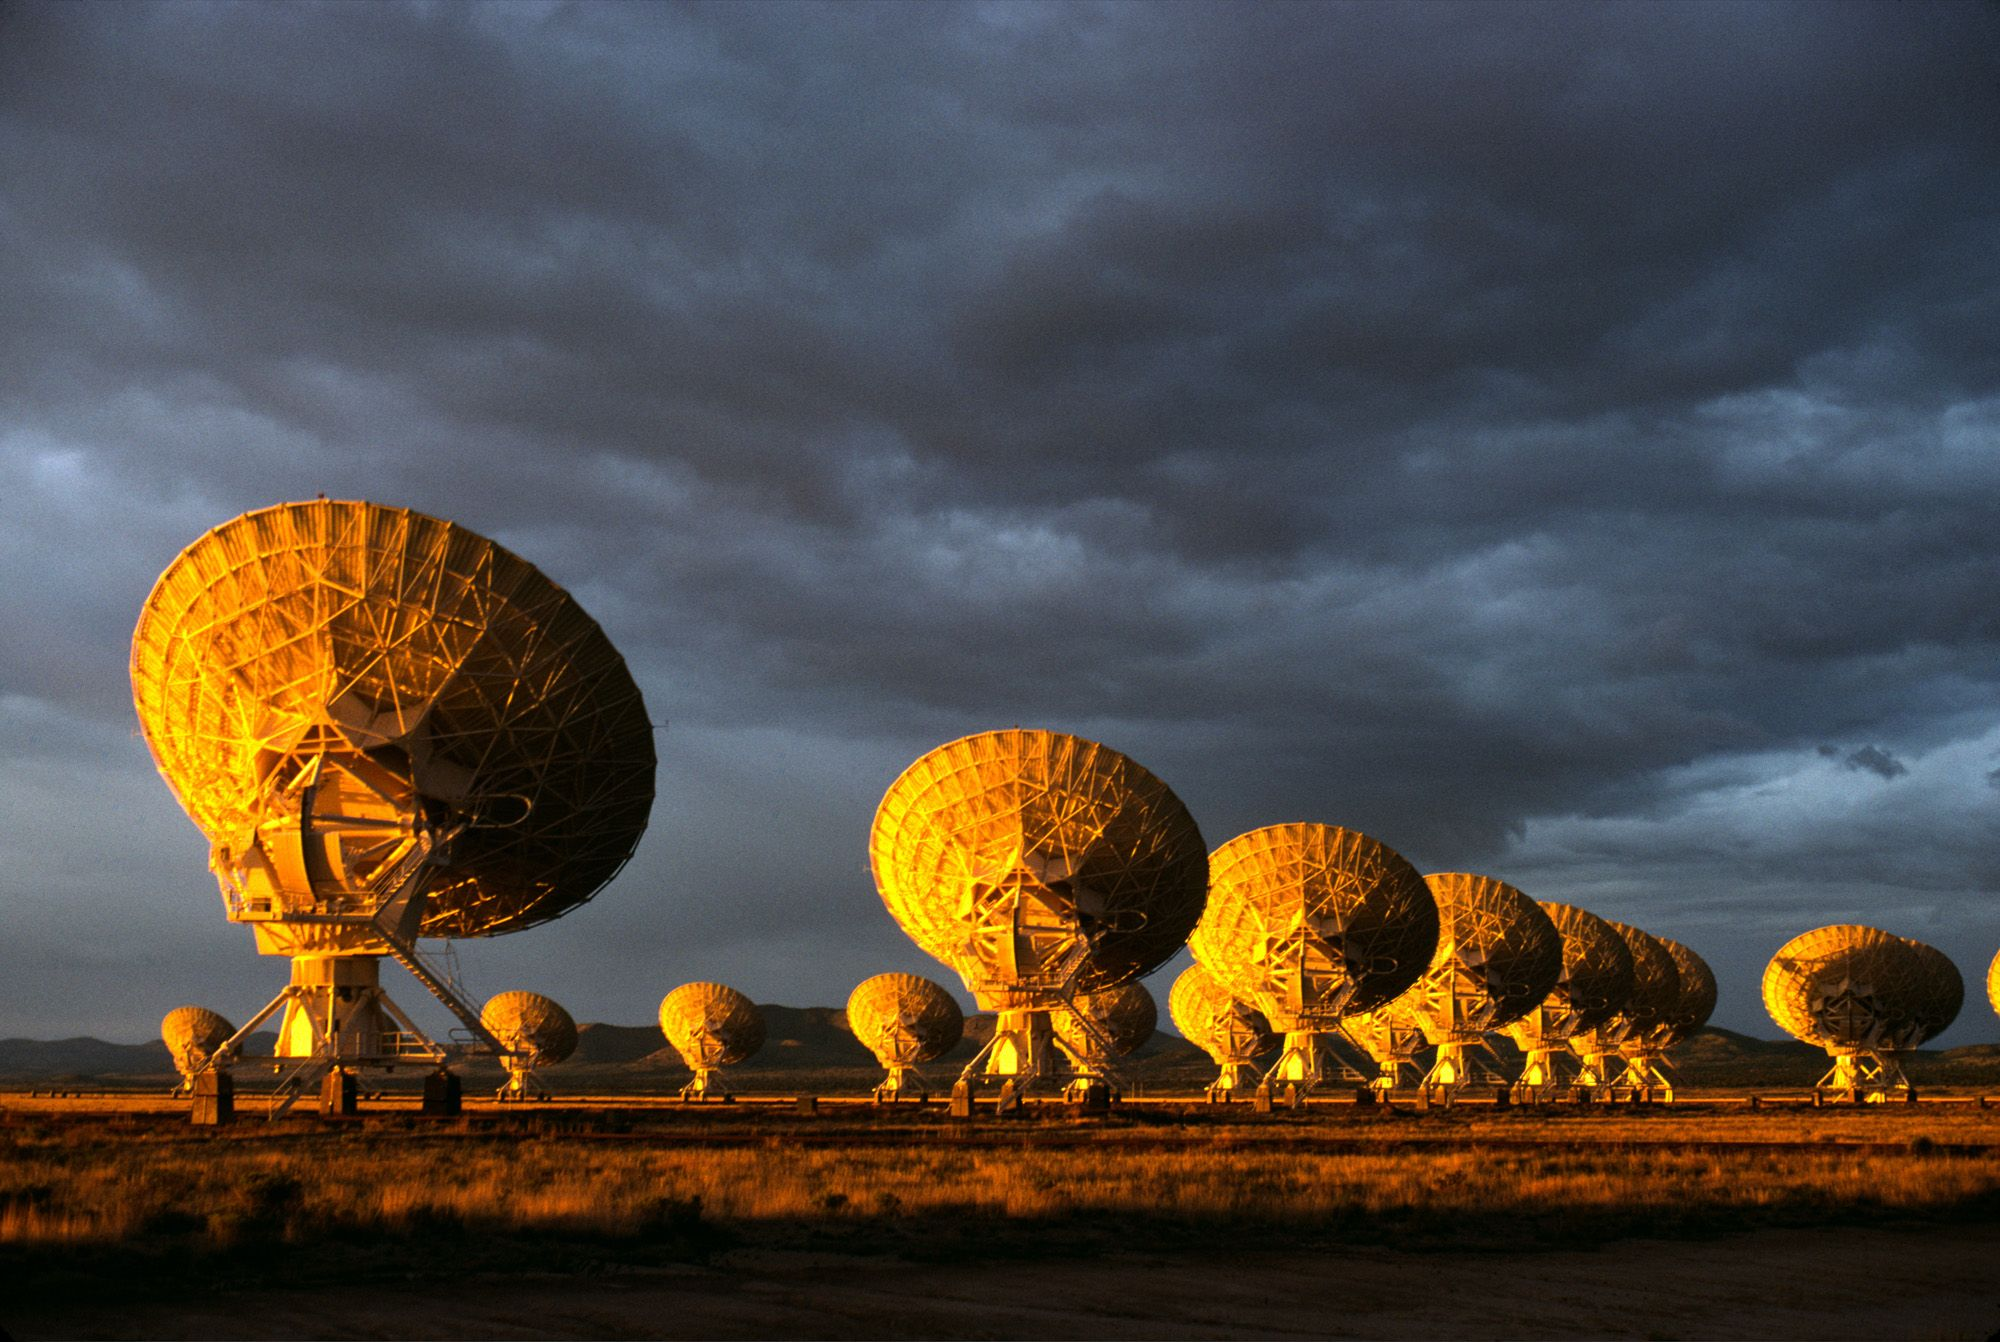
\includegraphics{at2019fdr/vla.jpg}
    \caption[VLA]{VLA in New Mexico. Image credit: NSF.}
    \labfig{vla}
\end{marginfigure}

In all three epochs, we did measure flux from the source location. Furthermore, the flux density declined with higher frequencies in all epochs. While epoch 1 and 2 showed no evolution in the \SIrange{4}{8}{\giga\Hz} and \SIrange{8}{12}{\giga\Hz} bands, the final epoch was suggestive of reduced flux and subsequently a spectral steepening in these bands. Intensive testing revealed that the reduced flux was not intrinsic to the source, but rather stemmed from significant atmospheric phase changes between the calibrator scans. These reduced the measured flux densities during epoch 3 due to decorrelation. As the source flux density was too low for self-calibration, the effect could not be corrected. We concluded that no evidence for temporal evolution in the radio can be found during the 5 months of observation. All measurements are shown in Fig.~\ref{fig:at2019fdr_radio} and listed in Table~\ref{tab:at2019fdr_radio}.

\begin{figure}[htb]
    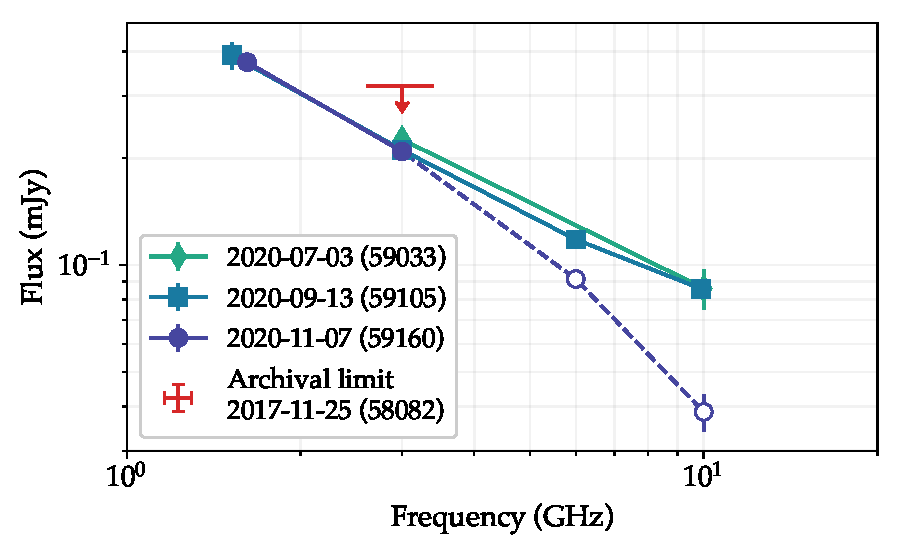
\includegraphics{at2019fdr/at2019fdr_radio.pdf}
    \caption[\emph{AT2019fdr} radio observations]{Radio observations of \emph{AT2019fdr}. An archival upper limit is shown in red. The apparent spectral steepening in the third epoch (dashed blue lines) are a calibration artifact from decorrelation due to atmospheric phase changes, and are not intrinsic to the source. Figure by the author, from~\cite{Reusch2022}.}
    \labfig{at2019fdr_radio}
\end{figure}

To compare to pre-flare host radio emission, we also obtained an archival upper limit from the Very Large Array Sky Survey (VLASS)~\sidecite{Lacy2020}. We exclusively used VLASS, as it was the only survey with sufficient sensitivity and angular resolution to probe \emph{AT2019fdr}. The quicklook continuum \texttt{fits} file for tile T17t23We was obtained from the archive\sidenote{\url{https://archive-new.nrao.edu/vlass/quicklook}}. The observation was carried out on November 25, 2017 in the \SIrange{2}{4}{\giga\Hz} band. At a significance level of \SI{3}{\sigma}, no emission from the source was detected. The local RMS noise was $\sigma=\SI{0.11}{\milli\jansky}/\text{beam}$, and the beam size was $\SI{2.46}{\arcsec} \times \SI{2.28}{\arcsec}$ at a position angle of \SI{-37}{\degree}. This resulted in an upper limit of \SI{0.32}{\milli\jansky}. A second VLASS observation was taken a few days prior to our second trigger epoch, but the resulting \SI{3}{\sigma} upper limit was less constraining (\SI{0.4}{\milli\jansky})~\cite{Reusch2022}.

\section{Near-infrared Observations}\label{nir_reductions}
After the detection of the neutrino, I triggered near-infrared (NIR) observations to extend the SED to longer wavelengths. We observed during four epochs with WIRC on the Palomar P200 in the \textit{J}-, \textit{H} and \textit{Ks}-band, centered on \SI{1.2}{\micro\m}, \SI{1.6}{\micro\m} and \SI{2.1}{\micro\m}. The dates of observations were July 1 and September 27, 2020, as well as February 2 and May 28, 2021.

All WIRC measurements were reduced using a custom pipeline (see~\sidecite{De2020}), which performs flat fielding, background subtraction and fits an astrometric solution using \textit{Gaia} DR2. Subsequently, the individual images for each filter and epoch were stacked to increase the signal-to-noise ratio. The photometric zero-point calibration of the stacked images was achieved within the pipeline by comparison to the Two Micron All Sky Survey (2MASS)~\sidecite{Skrutskie2006}.

\subsection{\texttt{GALFIT} flux extractions}

As another galaxy lies close to \emph{AT2019fdr}'s host galaxy (angular separation: \SI{7}{\arcsec}), I performed a manual flux extraction with \texttt{GALFIT}~\sidecite{Peng2002}. This two-dimensional fitting algorithm allows to define different galactic types and components, as well as point sources, and simultaneously fit the science images with these source types.

To improve photometric accuracy, I first derived the point spread function\sidenote{See Section~\ref{psfphot}} of individual stacked images with \texttt{photutils}~\sidecite{Bradley2020}, a package for the Python astronomy toolkit \texttt{astropy}~\sidecite{PriceWhelan2022}. All stars within the surrounding of \emph{AT2019fdr} were selected for this. From this selection, I visually selected a subset of stars neither too dim nor too bright (see Fig.~\ref{fig:at2019fdr_nir_starselection} for an example). Using these stars, I calculated the PSF of the image.

\begin{figure*}[htb]
    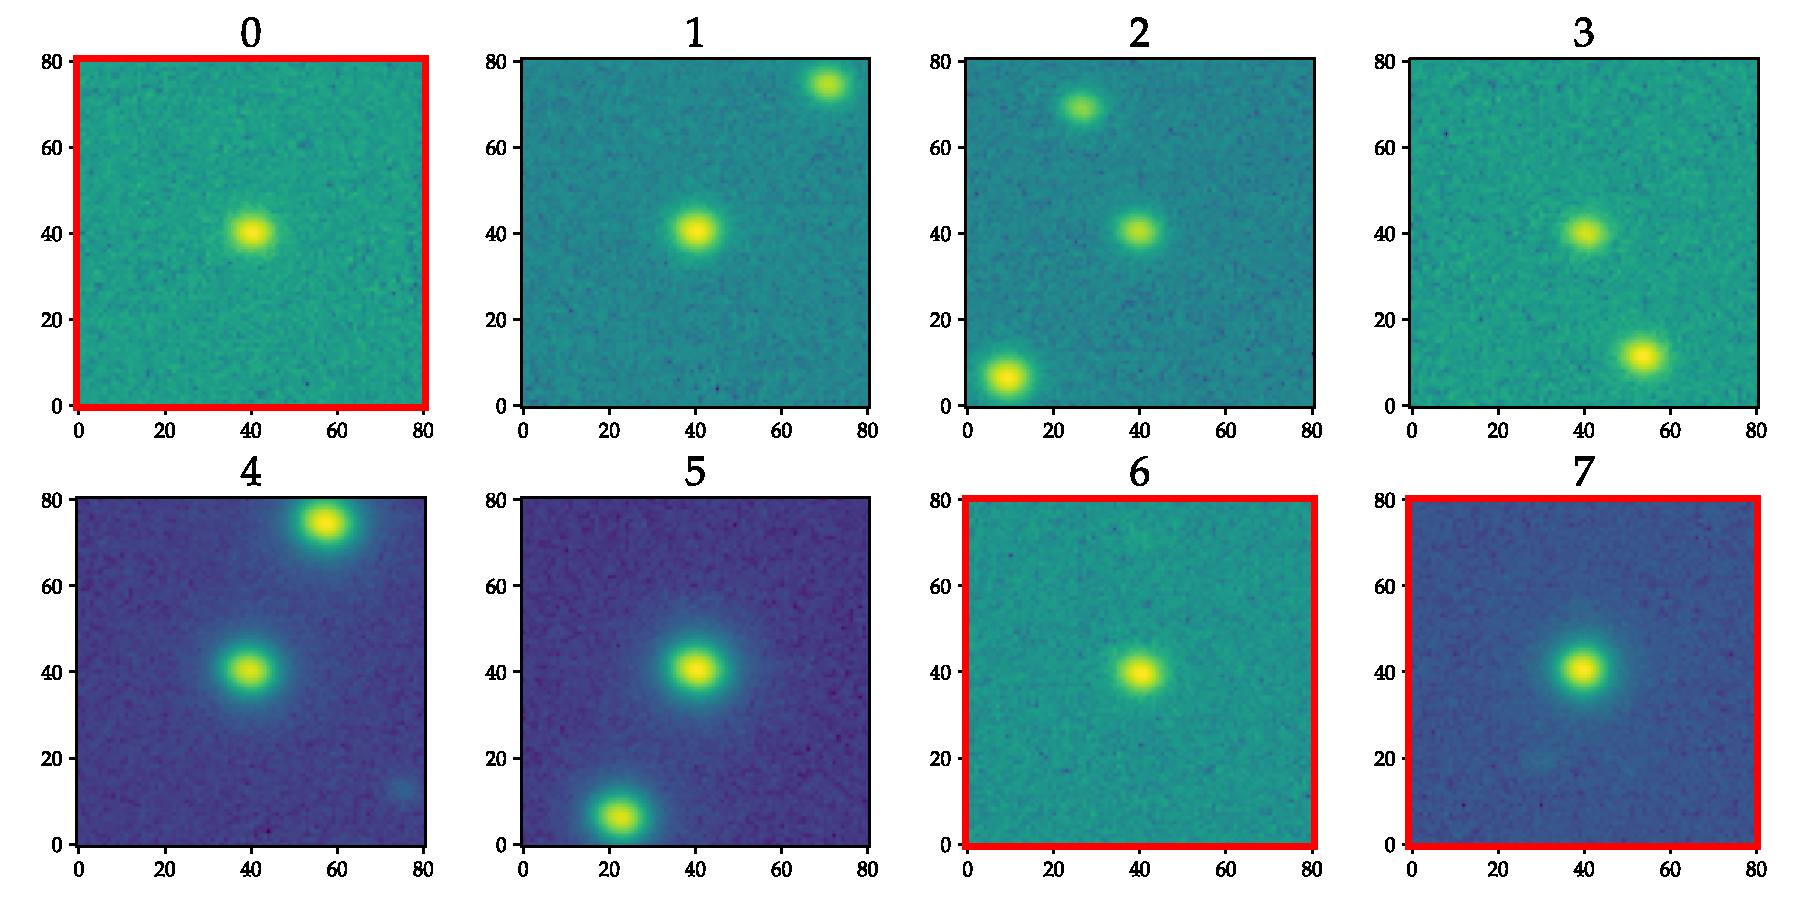
\includegraphics{at2019fdr/P200_third_epoch_H_stargrid.pdf}
    \caption[P200 \textit{H}-band star selection]{Star selection to fit the PSF of the stacked P200/WIRC \textit{H}-band image from Februar 2, 2021. Each cutout comprises $80\times80$ pixels. As can be seen, some of the stars have neighboring stars. As this can hamper a clean extraction of the PSF, such stars were rejected. All stars included in the PSF extraction are marked with a red rectangle (star 0, 6 and 7). One can also see that during this epoch observing conditions were not ideal, resulting in horizontally elongated images of the stars.}
    \labfig{at2019fdr_nir_starselection}
\end{figure*}

I retrieved the stars with \texttt{DAOStarFinder}, while I used \texttt{EPSFBuilder} for fitting the PSF. I verified the quality of the extracted PSF by inspecting the residuals of 4 nearby reference stars from SDSS (see Fig~\ref{fig:at2019fdr_nir_teststar}).

\begin{figure}[htb]
    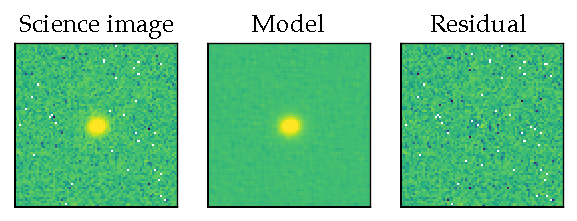
\includegraphics[width=0.8\textwidth]{at2019fdr/H_3_teststar2.pdf}
    \caption[P200 \textit{H}-band reference star]{P200 \textit{H}-band reference star. The \texttt{GALFIT} point source model constructed from the image PSF (center) was subtracted from the science image (left), with the residual shown on the right.}
    \labfig{at2019fdr_nir_teststar}
\end{figure}

I then ingested the resulting PSF into \texttt{GALFIT}. Two Sérsic  profiles describing the galaxy flux as a function of the distance to the galaxy core were then defined\sidenote{For details, see e.g.~\cite{Graham2005}.}, centered on the host and the neighboring galaxy location. Additionally, I used a point source with variable position to account for the transient flux. These three sources were then fit together, resulting in flux values for the host galaxy, the neighboring galaxy and the transient.

I fixed all parameters except for the point source flux after fitting one epoch (reference epoch). The point source flux was then fit in the remaining three epochs. Unfortunately, the choice of reference epoch had an impact on the point source flux values. This can be explained by differing observing conditions at different epochs. To account for this variation, both epoch 1 and epoch 4 were used as reference epochs. I used the difference in the resulting transient flux (when using epoch 1 as reference epoch on the one hand, and when using epoch 4 as such on the other hand) as systematic uncertainty on the extracted transient flux~\cite{Reusch2022}.

As there was no image without transient flux available, I added the point source flux to the host galaxy flux, and then subtracted the synthetic host model\sidenote{See Section~\ref{synthetic_host_model}.}. The model-subtracted AB magnitudes derived by this procedure are shown in Table~\ref{tab:p200_nir}.

\subsection{\textit{WISE} Detections}

\begin{marginfigure}
    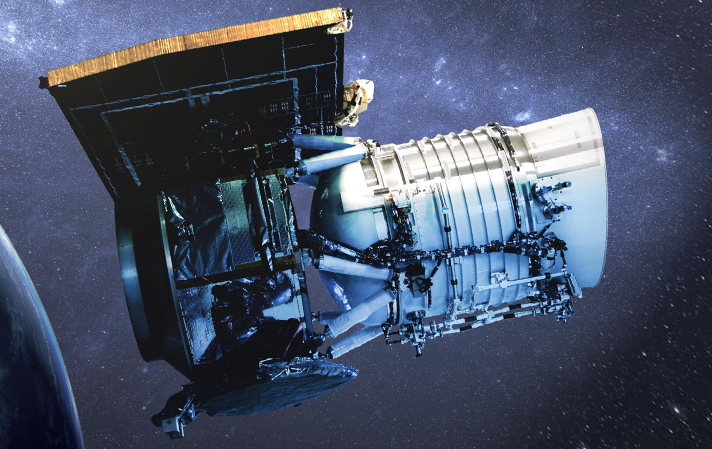
\includegraphics{at2019fdr/wise.jpg}
    \caption[The \textit{WISE} satellite]{The \textit{WISE} satellite. Image credit: NASA.}
    \labfig{wise}
\end{marginfigure}

Additionally to the ground-based NIR observations with P200, images from the mid-infrared (MIR) \textit{WISE} satellite were obtained in the \textit{W1}- and \textit{W2}-band (\SI{3.4}{\micro\m} and \SI{4.6}{\micro\m}).\ \textit{WISE} has cadence of 6 months, and the available images comprised 13 observational epochs prior to the detection of \emph{AT2019fdr}, as well as 3 epochs during the transient's life.

\pagebreak

As the \textit{WISE} MIR photometry---like the NIR photometry detailed above---suffered from blending with the nearby galaxy, forced PSF photometry was used on the co-added images (done with \texttt{ICORE}~\sidecite{Masci2013}) of each observational epoch. The package employed for this was \texttt{PythonPhot}~\sidecite{Jones2015}, a Python adaptation of the \texttt{DaoPhot}~\cite{Stetson1987} package.

The root mean square (RMS) of the pre-flare datapoints was only \SI{18}{\micro\jansky}, which was significantly smaller than the peak difference flux, measured at \SI{0.9}{\milli\jansky}. A robust baseline can therefore be constructed from the pre-flare \textit{WISE} detections.

\begin{figure}[htb]
    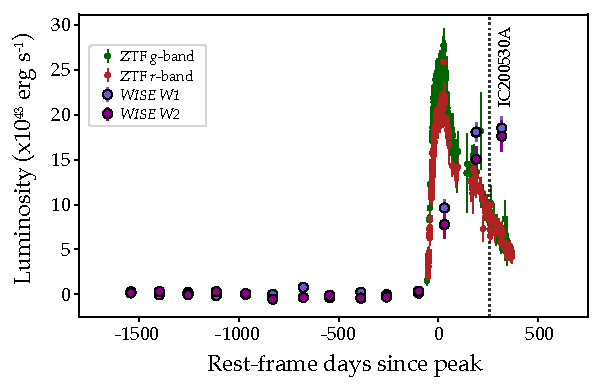
\includegraphics[width=1\textwidth]{at2019fdr/at2019fdr_wise.pdf}
    \caption[\textit{NEOWISE} forced photometry]{\textit{NEOWISE} + ZTF forced photometry light curve at the location of \emph{AT2019fdr}. The arrival time of neutrino \emph{IC200530A} is marked with a dotted black line. Note the small scatter of the pre-flare datapoints, allowing the construction of a robust baseline. From~\cite{Velzen2021}}
    \labfig{at2019fdr_wise}
\end{figure}

\subsection{Synthetic Host Model}\label{synthetic_host_model}
As not all measurements from the various instruments had the luxury of readily available reference images for easy extraction of transient light (as is e.g.\ the case for ZTF), we constructed a synthetic model of the host galaxy SED, which can be seen in Fig.~\ref{fig:host_model}. The best-fit values were a galaxy mass of $\log(M/M_\odot)=10.5$, a metallicity of $\log(Z/Z_\odot)=0.1$, dust extinction of $E(B-V)=1$, a star formation start time of $t=\SI{1.6}{\giga\year}$ after the Big Bang, and a star formation rate e-folding time of $\tau=\SI{0.8}{\giga\year}$.

The fit procedure is described in~\sidecite{Velzen2020}; we used archival measurements from different sources: To measure the UV flux, we used images from the Galaxy Evolution Explorer (\textit{GALEX})~\sidecite{Martin2005}. The \texttt{gPhoton}~\sidecite{Million2016} package with an aperture of \SI{4}{\arcsec} was used for flux extraction.

To measure the optical flux, we employed the model magnitudes from SDSS. These are computed either from a de Vaucouleurs galaxy profile, or an exponential galaxy profile, with \texttt{mag\_model} using the better of the two fits (see \url{https://www.sdss4.org/dr12/algorithms/magnitudes/mag_model} for details).

Lastly, we included the baseline \textit{WISE} datapoints detailed above, as well as an archival infrared measurement from the UKIRT Infrared Deep Sky Survey (UKIDSS)~\sidecite{Lawrence2007}.

\pagebreak

After gathering archival flux measurements from these sources, the \texttt{prospector} toolkit~\sidecite{Johnson2021} was used to sample synthetic galaxy models built by Flexible Stellar Population Synthesis (\texttt{FSPS})~\sidecite{Conroy2010}. This package is written in Fortran and was employed via the Python wrapper \texttt{python-fsps}~\sidecite{ForemanMackey2014}.

The archival values used in constructing the synthetic host model can be found in the Appendix in Table~\ref{tab:host_model_measurements}.

\begin{figure}[htb]
    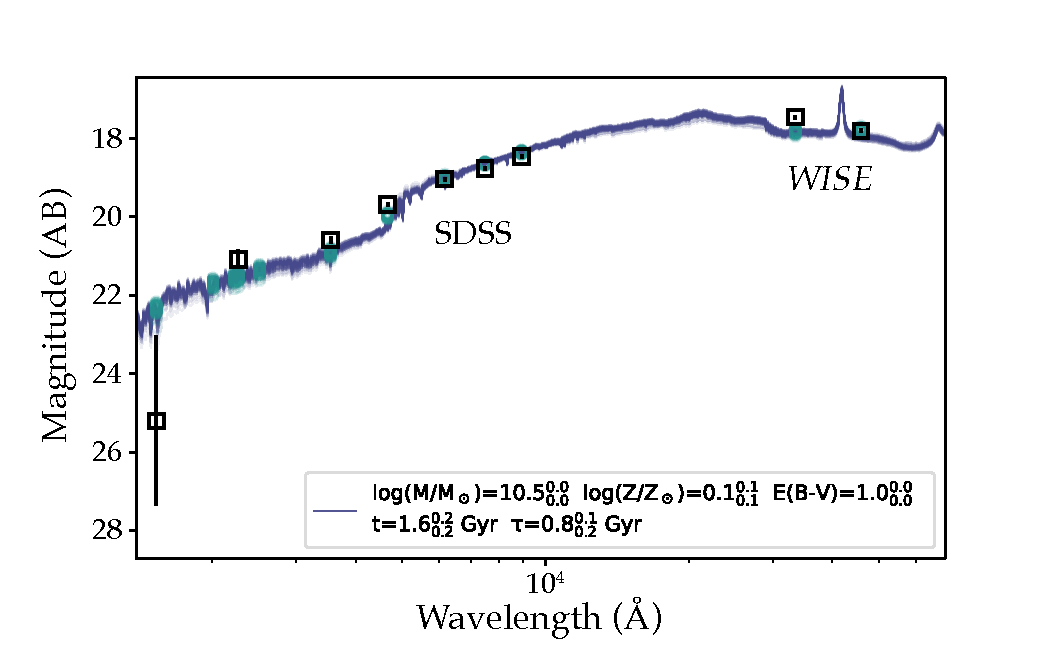
\includegraphics[width=1\textwidth]{at2019fdr/host_model.pdf}
    \caption[Synthetic host spectrum]{Synthetic host spectrum constructed with \texttt{FSPS}. Figure by S. van Velzen, annotations by the author.}
    \labfig{host_model}
\end{figure}

I subsequently subtracted the host model from all measurements possibly containing host light within their respective bandpass using \texttt{SNCosmo}~\sidecite{Barbary2022}, a Python framework dedicated to supernova analysis.

\begin{table}
    \centering
    \begin{tabular}{c c c c  c}
        \hline
        \textbf{MJD} & \textbf{Date} & \textbf{\textit{J}-band} & \textbf{\textit{H}-band} & \textbf{\textit{Ks}-band} \\
                     &               & (\SI{1.2}{\micro\m})     & (\SI{1.6}{\micro\m})     & (\SI{2.1}{\micro\m})      \\
        \hline
        \hline
        59031        & 2020--07--01  & $19.06 \pm 0.50$         & $ 17.73 \pm 0.12$        & $17.13 \pm 0.26$          \\
        59121        & 2020--09--29  & $19.78 \pm 0.98$         & $ 17.76 \pm 0.12$        & $17.45 \pm 0.35$          \\
        59249        & 2021--02--04  & ---                      & $ 18.26 \pm 0.19$        & $17.81 \pm 0.48$          \\
        59362        & 2021--05--28  & ---                      & $ 18.42 \pm 0.22$        & $17.91 \pm 0.53$          \\
        \hline
    \end{tabular}
    \caption[NIR magnitudes]{NIR AB magnitudes after subtracting the synthetic host model. Only systematic uncertainties are provided, as the photometric uncertainties should be negligible in comparison, at least in the \textit{J}- and \textit{H}-band. The flux of the third and fourth \textit{J}-band epochs after host-model subtraction was negative, which was counted as non-detection. From~\cite{Reusch2022}}\label{tab:p200_nir}
\end{table}

\section{SED Blackbody Modeling}
After compiling and reducing the individual light curve measurements, a physical model motivating the detected light needed to be applied.

To explain the SED, I employed different models: A power law, a single blackbody, a broken power law\sidenote{I.e.\ a power law with a break at a certain wavelength where the spectral index changes.} and lastly a double blackbody model. In the following, the derivation of this model and the energy output of the system described by it will be detailed, including a discussion of dust extinction.

\subsection{Fit Epochs}
For the fit I isolated three regions of interest. These comprised (1) the 20 days between August 5 and 25, 2019, as this windows covered the optical peak of the light curve, as well as the first \textit{WISE} measurement. The second, longer epoch (2) ranged from June 6 to October 8, 2020 (124 days), shortly after the neutrino detection. It covered one \textit{WISE} measurement epoch and two P200 NIR observations. The last epoch (3) covered January 1 to February 26, 2021 (51 days) and contained another P200 NIR observation.

As the light curve did not significantly change within those epochs, I used the mean flux values for each observed bands as input for the fitting procedure.

\subsection{Fit Models}\label{fitmodels}
As stated above, I tried a variety of models of increasing complexity. The least complex model that captured the measurements reasonably well was a double blackbody model. These models were, with increasing number of free parameters:

\begin{description}
    \item[Unbroken power law] A single, unbroken power law with the power law index as free parameter.
    \item[Single blackbody] This model is described by two parameters, the blackbody radius and its temperature.
    \item[Broken power law] The two spectral indices and the wavelength of the break are the free parameters here.
    \item[Double blackbody] Two unmodified blackbodies, resulting in four free parameters ($2 \times$ temperature, $2 \times$ radius).
\end{description}

All fits were performed with the \texttt{lmfit}~\sidecite{Newville2021} Python package, which implements the Levenberg-Marquardt algorithm for solving non-linear least-squares problems.

To account for host extinction, I used the \texttt{extinction}~\sidecite{Barbary2016} Python package, namely the Calzetti attenuation law~\sidecite{Calzetti2000} contained therein. I fixed the extinction $R_V$ at 3.1, the value typical for the Milky Way~\sidecite{Schultz1975} and left $A_V$ free in epoch 1. The best-fit value of $A_V=0.45^{+0.14}_{-0.14}$ was fixed in epoch 2 and 3. I decided on using epoch 1 to determine $A_V$ as it provided the best optical and UV coverage of the three epochs. For the double blackbody model, this procedure ultimately resulted in 5 (4) free parameters in epoch 1 (2 and 3).

I imported the measurements, averaged the flux in each band per epoch, and passed them to the minimizer (the fit priors are shown in Table~\ref{tab:double_bb_priors}).

\begin{table}
    \begin{center}
        \begin{tabular}{c c c}
            \hline
            \textbf{Parameter} & \textbf{Initial value} & \textbf{Bounds}                 \\
            \hline
            \hline
            $A_V$              & $0.45$                 & $[0, 2]$                        \\
            $T_1$              & \SI{1730}{\K}          & [\SI{7000}{\K}, \SI{50000}{\K}] \\
            $T_2$              & \SI{1650}{\K}          & [\SI{500}{\K}, \SI{2300}{\K}]   \\
            $S_1$              & \num{2.3e23}           & [\num{1e20}, \num{1e27}]        \\
            $S_2$              & \num{1e20}             & [\num{1e18}, \num{1e21}]        \\
            \hline
        \end{tabular}
    \end{center}
    \caption[Double BB fit priors]{Priors for the double blackbody minimization. $A_V$ is the extinction parameter (only fitted in epoch 1 and fixed for epoch 2 and 3), $T_1$ and $T_2$ are the temperatures of the two blackbodies, while $S_1$ and $S_2$ are the `Scale' parameters (which can be converted into radii.)}\label{tab:double_bb_priors}
\end{table}

The model for the blackbodies was provided by \texttt{astropy}\sidenote{\texttt{astropy.modeling.models.BackbBody}}. As this model works with a \textit{scale} parameter\sidenote{This \texttt{astropy} terminology is slightly confusing, as the scale has units of spectral radiance (\unit{\erg\per\s\per\square\cm\per\Hz\per\steradian}).} instead of a blackbody radius, this needed to be converted via

\begin{equation}
    \text{Scale} = d_L^2 / (r^2 \pi)
\end{equation}

where $r$ is the blackbody radius and $d_L$ is the luminosity distance, calculated with the redshift $z=0.2666$ and assuming a standard cosmology. The luminosity distance is a measure for how far away something `looks'. If the luminosity $L$ is the total amount of energy isotropically radiated by an object per unit time, it is related to the flux $F$ measured at luminosity distance $d_L$ via this relation, describing an expanding sphere of light:

\begin{equation}
    d_L = \sqrt{L/4\pi F}
\end{equation}

The luminosity distance is equal to the proper distance (as in the amount of space a photon had to traverse to reach us) if and only if the universe is geometrically flat and the universe is static, so it is neither shrinking nor expanding. As the universe in fact \textit{is} expanding, the luminosity distance is similar to the proper distance only for small redshifts (i.e.\ if there was little time needed for the photon to reach us, and therefore little expansion). In general, the luminosity distance depends on the evolution of the universe. Here, I calculated the luminosity distance with the \texttt{astropy.cosmology} module.

\subsection{Minimization}

\begin{figure*}[htb]
    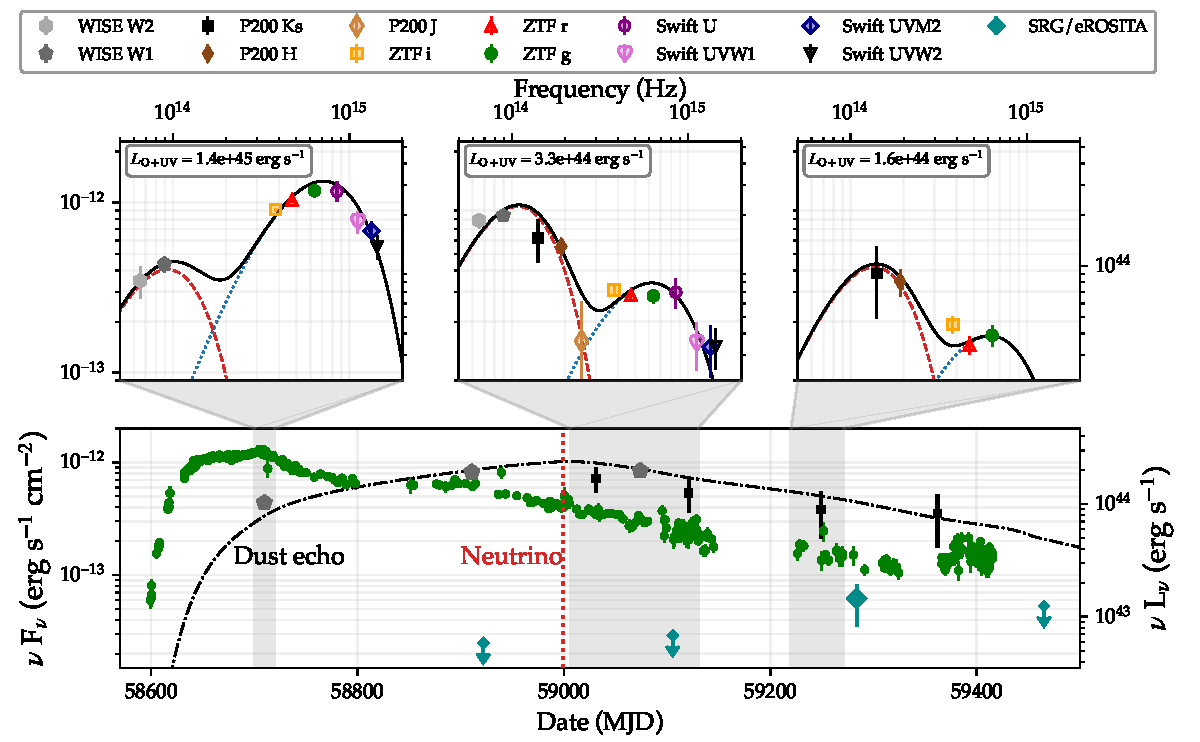
\includegraphics{at2019fdr/at2019fdr_lightcurve_and_sed.pdf}
    \caption[\emph{AT2019fdr} light and SED]{Light curve and SED of \emph{AT2019fdr}. The three panels on the top show the double blackbody fits for the three epochs marked in light gray. On the bottom, the ZTF \textit{g}- and \textit{WISE W1}-band light curve is shown (green circles and gray pentagons), alongside the P200 \textit{Ks} band data (black squares) as well as the three upper limits and one X-ray detection by \textit{SRG}/eROSITA (rotated cyan squares), and the modeled dust echo emission (black dash-dotted line). The left y-axes show $\nu F_\nu$ (where $F_\nu$ is the spectral flux density at frequency $\nu$), and the right y-axes display $\nu L_\nu$ (with $L_\nu$ being the luminosity at frequency $\nu$). Figure by the author, from~\cite{Reusch2022}.}
    \labfig{at2019fdr_lightcurve_and_sed}
\end{figure*}

In each iteration of the minimization process, the spectrum of both blackbodies constructed as such were then reddened, and redshifted. After this, the flux of the two blackbody spectra was added up.

To extract the flux as observed in each band, I used \texttt{SNCosmo} to evaluate all bands given their transmission function. For this I ised the integrated bandpass library of \texttt{SNCosmo}. Bandpasses that were not shipped with the package were added manually from the SVO Filter Profile Service~\sidecite{Rodrigo2020}. This was the case for \textit{Swift}, P200 and \textit{WISE}.

The best fit values from all three epochs, as well as their uncertainties at the \SI{68}{\percent} confidence level can be seen in Table~\ref{tab:double_bb}. The best-fit temperatures resulted in a `blue' blackbody peaking in optical/UV wavelengths, and a `red' blackbody peaking in the infrared.

I derived an optical/UV peak luminosity of $L=\SI[parse-numbers = false]{1.4^{+0.1}_{-0.1}\times10^{45}}{\erg\per\s}$. By integrating this component over time by scaling it with the shape of the ZTF \textit{g}-band light curve, I obtained a total bolometric luminosity of $E_\text{bol} = \SI{3.4e52}{\erg}$. I did not add the infrared blackbody, as dust absorption was already accounted for by fitting for dust extinction. This pushed \emph{AT2019fdr} to the class of brightest transients ever detected. Its inferred bolometric energy was almost twice as high as that of ASASSN-15lh, which was one of most luminous transients ever reported~\sidecite{Dong2016} and which was suggested to be a TDE~\sidecite{Leloudas2016}.

\begin{table}
    \renewcommand{\arraystretch}{1.3}
    \centering
    \begin{tabular}{c c  r  c  c}
        \hline
        \textbf{Epoch} & \textbf{Band} & \textbf{Temp.}           & \textbf{Radius}                     & \textbf{Luminosity}                 \\
                       &               & (\unit{\K})              & (\unit{\cm})                        & (\unit{\erg\per\s})                 \\
        \hline
        \hline
        \textbf{1}     & O+UV          & $ 13526^{+569}_{-574}$   & $ 7.8^{+0.4}_{-0.4} \times 10^{15}$ & $ 1.4^{+0.1}_{-0.1} \times 10^{45}$ \\
                       & IR            & $1505^{+421}_{-313}$     & $ 2.2^{+1.6}_{-1.4} \times 10^{17}$ & $1.7^{+2.2}_{-1.0} \times 10^{44}$  \\
        \hline
        \textbf{2}     & O+UV          & $ 11731^{+663}_{-683}$   & $ 4.9^{+0.4}_{-0.4} \times 10^{15}$ & $ 3.3^{+0.3}_{-0.4} \times 10^{44}$ \\
                       & IR            & $1762^{+121}_{-124}$     & $ 2.5^{+0.2}_{-0.2} \times 10^{17}$ & $4.3^{+0.5}_{-0.7} \times 10^{44}$  \\
        \hline
        \textbf{3}     & O+UV          & $ 10230^{+2373}_{-1645}$ & $ 4.3^{+3.3}_{-1.0} \times 10^{15}$ & $ 1.5^{+1.2}_{-0.4} \times 10^{44}$ \\
                       & IR            & $2237^{+402}_{-462}$     & $ 1.0^{+0.6}_{-0.4} \times 10^{17}$ & $1.9^{+1.4}_{-0.5} \times 10^{44}$  \\
        \hline
    \end{tabular}
    \caption[Blackbody best-fit values]{Blackbody best-fit values for three epochs (1--3).\ \textit{O+UV} denotes the `blue' blackbody in the optical/UV and \textit{IR} denotes the `red' infrared blackbody. The luminosity is given dereddened and in the source frame. The uncertainties are at the 68\% confidence level. Note that the O+UV temperature and radius (and therefore the luminosity) in the third epoch are not well constrained, as no late-time UV measurements were available. The same holds true for the IR blackbody in the first and the last epoch, as only two data points were available.}\label{tab:double_bb}
\end{table}


\subsection{Uncertainty Estimate}
As the fit routine was not able to generate stable covariance matrices in all epochs, the I estimated the uncertainties manually.

\begin{marginfigure}
    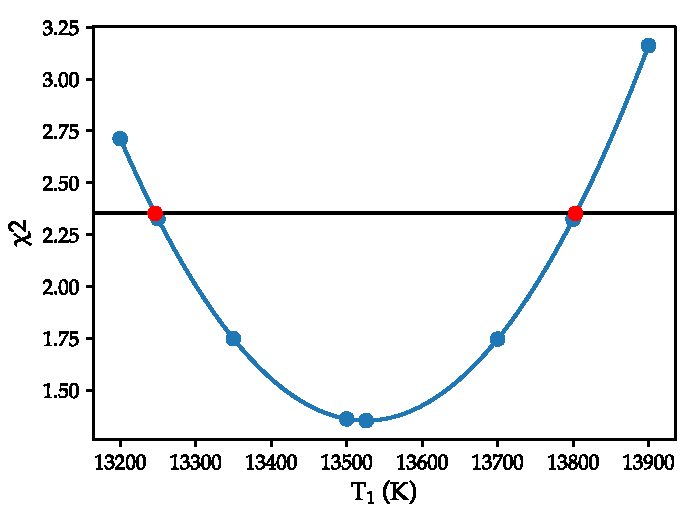
\includegraphics{at2019fdr/at2019fdr_bb_chisq.pdf}
    \caption[Uncertainty estimation for double BB fit]{Uncertainty estimation for the double blackbody fits. Here, the uncertainty of the temperature $T_1$ of the hot (blue) blackbody during epoch 2 is estimated. The red datapoints mark the \SI{68}{\percent} confidence level.}
    \labfig{bb_chisq}
\end{marginfigure}

For each epoch and fit parameter, this was done by letting all parameters vary except for the parameter of interest. I then varied this parameter around the best-fit value, and the resulting $\chi^2$ was evaluated. Following this, I approximated the $\chi^2$ distribution with a polynomial, and calculated the \SI{68}{\percent} confidence level---the two parameter values with $\chi^2 - \chi^2_\text{min} = 1$ confine the \SI{68}{\percent} confidence level.

From the fit parameter uncertainties calculated as such, I obtained uncertainties on the radius and the luminosities via Gaussian error propagation.

\begin{figure}[htb]
    \centering
    \begin{subfigure}{0.48\textwidth}
        \centering
        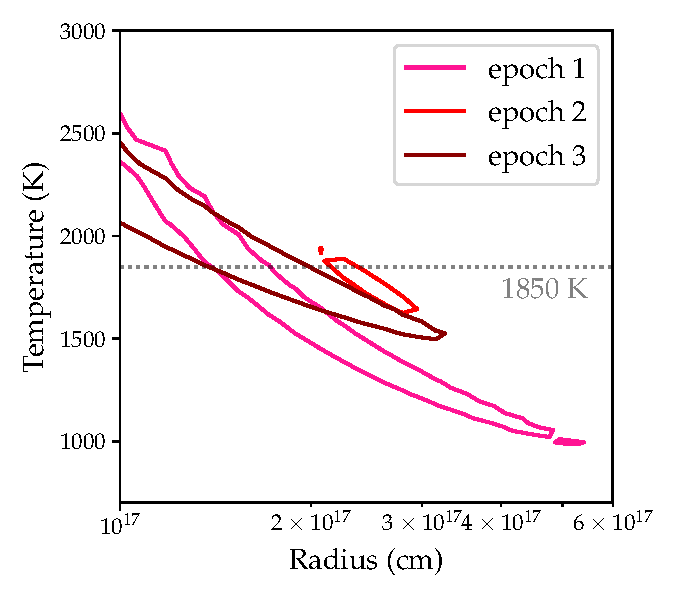
\includegraphics[width=0.95\textwidth]{at2019fdr/at2019fdr_contour_all.pdf}
        \caption{Infrared blackbody, \SI{90}{\percent} CL contours for all three epochs (optical+UV blackbody fit parameters remain free).}\label{fig:at2019fdr_contour_all}
    \end{subfigure}
    \hfill
    \begin{subfigure}{0.48\textwidth}
        \centering
        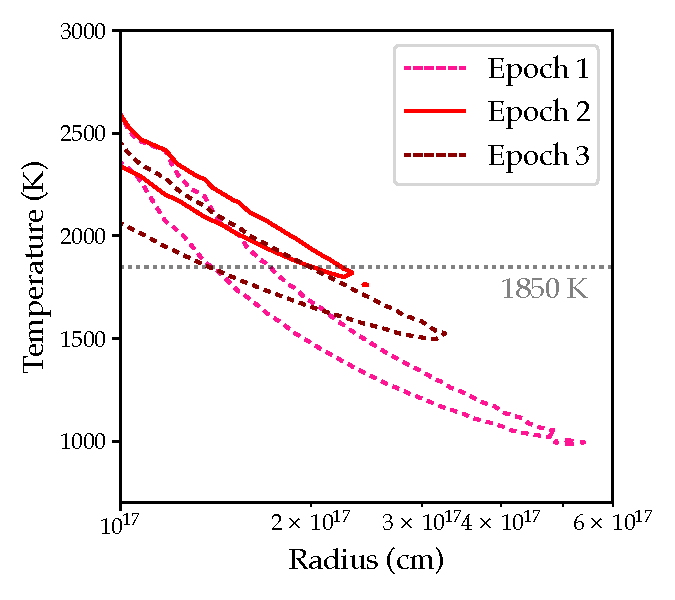
\includegraphics[width=0.95\textwidth]{at2019fdr/at2019fdr_contour_all_no_WISE.pdf}
        \caption{Infrared blackbody, \SI{90}{\percent} CL contours for all three epochs after removing the two \textit{WISE} datapoints for epoch 2.}\label{fig:at2019fdr_contour_all_nowise}
    \end{subfigure}
    \caption[\emph{AT2019fdr} temperature fit]{\SI{90}{\percent} CL contours for the infrared blackbody temperature fits, once including the \textit{WISE} data in all epochs (plot on the left), and once after removing them in epoch 2 (plot on the right). The contours of epoch 2 (solid red line) move to a region of higher temperatures comparable to epoch 3 when the \textit{WISE} datapoints are removed. This shows that they are pushing the temperature down.}\label{fig:at2019fdr_contour}
\end{figure}

As can be seen in Table~\ref{tab:double_bb}, the third epoch saw a temperature rise in the infrared blackbody. As these values were in tension with the dust-echo model discussed in the next Section~\ref{dust_echo}, I investigated this behavior.

The most likely reason for the higher temperature in epoch 3 is that the infrared blackbody was less constrained in that epoch, as there were no \textit{WISE} measurements available, and the P200 \textit{J}-band extraction resulted in a non-detection. In Fig.~\ref{fig:at2019fdr_contour_all}, one can see that all three epochs were compatible within their \SI{90}{\percent} confidence level with a blackbody temperature of \SI{1850}{\K}.

Furthermore, all epochs showed the expected linear correlation between increasing blackbody temperature and decreasing radius of the blackbody. Fig.~\ref{fig:at2019fdr_contour} shows how the \SI{90}{\percent} contour of epoch 2 gets moved to a higher temperature and lower radius when removing the two \textit{WISE} datapoints. This reinforces the case that the higher best-fit temperature in epoch 3 is merely an artifact of having less constraints for the fit and not some unexplained physical process.

\section{Dust Echo Model}\label{dust_echo}
As one can see in the light curve of \emph{AT2019fdr} (see Fig.~\ref{fig:at2019fdr_light_curve}), the emission in all infrared bands (\textit{WISE} and P200) is delayed with respect to the optical signal. Furthermore, the infrared emission is well approximated by a blackbody, as was shown in the last section.

As the infrared blackbody with a delayed increase in brightness with respect to the optical light curve is well explained by such a model, I interpreted this infrared emission as a dust echo. In this model, the X-ray to optical light from the flare is reprocessed by dust. This dust is usually located in a torus around the supermassive black hole (SMBH) at the center of the host galaxy~\sidecite{Velzen2016}. The high luminosity of the flare causes the dust in the vicinity of the black hole to evaporate, up to a safe distance, at which the incident flux heats the dust, but not above its sublimation temperature at around \SI{1850}{\K}.

Outside the sublimation radius, the grain temperature is coupled to the incident radiation, as it cools rapidly. The cooling time is $10^{-4} a_{0.1}^{-1}T_{1850}^{-5}\unit{\s}$, which equals to \SI{0.1}{\milli\s} for a grain size of \SI{0.1}{\micro\m} at \SI{1850}{\K}~\cite{Velzen2016}.

According to \cite{Velzen2016}, the infrared light curve produced this way can be approximated as follows:

\begin{equation}
    L_\text{IR} = \int d\tau~ \Psi(\tau) ~L(t-\tau),
\end{equation}

where $L(t)$ is the light curve of an isotropic flare,  $\Psi(\tau)$ is the response function and $\tau$ is the delay. In the case of a spherical dust shell, $\Psi(\tau)$ can be approximated by a square wave response function, ranging from $\tau=0$ to $\tau = 2 R_0 c$ (where $R_0$ is the radius of the dust shell). One can therefore write

\begin{equation}
    L_\text{IR} = \int d\tau L (t-\tau) ~\Pi (\tau),
\end{equation}
where $\Pi$ is the rectangular function
\begin{equation}
    \Pi(\tau) = \begin{cases}
        0           & \text{if $|\tau|>\frac{1}{2}$}   \\
        \frac{1}{2} & \text{if $|\tau| = \frac{1}{2}$} \\
        1           & \text{if $|\tau|<\frac{1}{2}$}.
    \end{cases}
\end{equation}
The delay induced by light travel time can thus be approximated by convolving the optical light curve with a rectangular function of width $2\times\Delta_{t_c}$, where $t_c$ is the light travel time from the transient to the surrounding dust sphere.

This can be understood if one looks at the geometry of the system. After a delay of $\Delta_{t_c}$, light from the flare reaches the inner edge of the sphere that survives the incident radiation, directly along our line of sight. Here it gets re-emitted in the infrared and reaches us with that initial delay of $cR_0$. Re-emitted light from the side of the system takes even longer. Lastly, re-emitted light from the back of the system reaches us with a delay of $3\times cR_0$---first the flare light needs to travel one radius away from us, and then the re-emitted light needs to cross the whole system (twice $R_0$) towards us.

To calculate $R_0$, I used the ZTF \textit{g}-band light curve, as it had the best sampling. I then convolved this light curve with the box function, where the width of the box function in days was left as free parameter. The initial delay with respect to the optical light curve was then half the size of the box function. The second free parameter was a dimensionless amplitude used to scale the optical light curve to match the amplitude of the \textit{WISE} datapoints.

Following this procedure, I obtained a best-fit light travel time of 193 days, which translates to $R_0=\SI{0.16}{\parsec}$. The best fit parameters can be seen in Fig.~\ref{fig:at2019fdr_dust_model_chisq} and result in the black dash-dotted curve in Fig.~\ref{fig:at2019fdr_lightcurve_and_sed}.

To crosscheck this result, I used the fact that according to~\cite{Velzen2016}, the radius of this dust shell can be approximated as
\begin{equation}
    R= \bigg(\frac{L_{45}}{a_{0.1}^2 T_{1850}^{5.8}} \bigg)^{1/2} \text{pc},
\end{equation}
where $L_{45}$ is the flare's luminosity integrated over all wavelengths where the dust absorbs, normalized to \SI{1e45}{\erg\per\s}, $a_{0.1}$ is the dust grain size normalized to $\SI{0.1}{\micro\m}$, and $T_{1850}$ is the grain temperature normalized to \SI{1850}{\K}.

\begin{figure}[htb]
    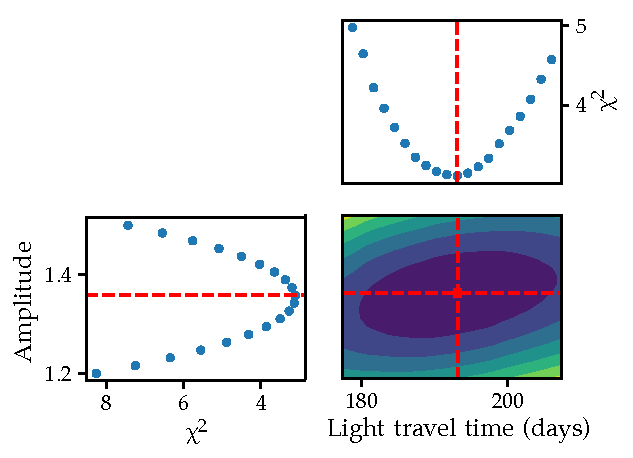
\includegraphics[width=0.8\textwidth]{at2019fdr/dust_model_chisq_simple.pdf}
    \caption[Dust model fit corner plot]{Corner plot of the dust model fit for \emph{AT2019fdr}. The two free parameters (dimensionless amplitude and light travel time in days) are plotted together with the marginalized $\chi^2$ values.}
    \labfig{at2019fdr_dust_model_chisq}
\end{figure}

When inserting the infrared blackbody temperature from the second epoch (as it is the best constrained one) with a temperature of \SI{1762}{\K}, using the default grain size and the peak optical luminosity of \SI{1.4e45}{\erg\s}, this equation yielded a sublimation radius of \SI{0.2}{\parsec}, which is in good agreement with the best-fit value of \SI{0.16}{\parsec}.

To obtain the covering factor, i.e.\ the fraction of the shell around the transient that actually containes dust, I needed to derive the total bolometric energy of the dust echo. This was achieved by time-integrating the fitted dust echo light curve, scaled to the peak luminosity of \SI{4.3e44}{\erg\s}. This resulted in a dust echo bolometric energy of \SI{1.1e45}{\erg}. The ratio of the the dust echo bolometric energy to the optical/UV bolometric energy yielded a covering factor of 1/3, assuming a \SI{100}{\percent} efficiency in the absorption-reemission process. This value was unusually high (TDEs in quiescent galaxies usually have covering factors \SI{\sim1}{\percent}, see~\cite{Velzen2016}). The high covering factor can be explained by the fact that---contrary to usual TDEs---the system is an active galactic core, with a pre-existing dust torus.

Lastly, I used this covering factor and the radius of the dust shell to determine the dust mass. Again assuming a grain size of \SI{0.1}{\micro\m}, spherical dust grains and a typical dust mass density of \SI{2.5}{\g\per\cm}~\sidecite{Mann2000} resulted in a mass of $0.017 ~\text{M}_\odot$ contributing to the echo. When assuming a typical mass-to-gas ratio of 1:100~\sidecite{Leroy2011}, this corresponds to $1.7 ~\text{M}_\odot$ in gas.

\section{Classification}
As stated at the beginning of this chapter, \emph{AT2019fdr} was initially classified as a SLSN IIn, but a subsequent paper classified \emph{AT2019fdr} as TDE~\cite{Frederick2021}. In this section I will present their reasoning, as well as further evidence we brought forward in favor of this hypothesis, but also some data weakening this interpretation.

\subsection{Original TDE Classification}
Frederick et al.~\cite{Frederick2021} outright rejected the initial SLSN IIn interpretation, but discussed that \emph{AT2019fdr}---like all the 5 flares located in NLSy1 galaxies they studied---could either be an AGN flare or a TDE. They based their classifications on a set of criteria, detailed in Table~\ref{tab:at2019fdr_classification_matrix}. The green cells in the table show that the feature being present (\checkmark) or absent ($\times$) makes a TDE interpretation more likely, while red color means that it renders a flare origin more likely. For comparison, \textit{AT2019dsg} is shown as an example of a bona fide TDE.

\begin{table*}[htp]
    \begin{center}
        \begin{tabular}{c c c c c c c c c c}
            \hline
            Name              & $M_\text{BH}<$              & $\text{H}_\beta<2000$     & FeII                      & [OIII]$/\text{H}_\beta$   & $\Delta g-r$                & UV                          & X-ray                         & \textit{W1}-\text{W2}     & Re-                       \\
                              & $10^8 M_\odot$              & \unit{\km\per\s}          &                           & $<3$                      & $\sim 0$ mag                &                             & \& $\Gamma$                   & $>0.7$ mag                & brighten                  \\
            \hline
            \emph{AT2019fdr}  & \cellcolor{green}\checkmark & \cellcolor{red}\checkmark & \cellcolor{red}\checkmark & \cellcolor{red}\checkmark & \cellcolor{red}$\times$     & \cellcolor{green}\checkmark & \cellcolor{green}$\times$     & \cellcolor{green}$\times$ & \cellcolor{green}$\times$ \\
            \emph{PS1--10adi} & \cellcolor{green}\checkmark & \cellcolor{red}\checkmark & \cellcolor{red}\checkmark & \cellcolor{red}\checkmark & \cellcolor{green}\checkmark & \cellcolor{green}\checkmark & \cellcolor{green}(\checkmark) & \cellcolor{green}$\times$ & \cellcolor{green}$\times$ \\
            \hline
            \hline
            \emph{AT2019dsg}  & \cellcolor{green}\checkmark & \cellcolor{red}\checkmark & \cellcolor{green}$\times$ & \cellcolor{red}\checkmark & \cellcolor{green}\checkmark & \cellcolor{green}\checkmark & \cellcolor{green}(\checkmark) & \cellcolor{green}$\times$ & \cellcolor{green}$\times$ \\
            \hline
        \end{tabular}
    \end{center}
    \caption[\emph{AT2019fdr}/\emph{PS1--10adi} classification matrix]{Classification matrix of \emph{AT2019fdr} and ambiguous transient \emph{PS1--10adi} for comparison, as well as bona fide TDE \textit{AT2019dsg}.\ \checkmark\ means the property is present, while $\times$ marks an absence.\ \textcolor{green}{Green} means that the presence or absence favors a TDE interpretation, while \textcolor{red}{red} is evidence for an AGN flare interpretation. (\checkmark) means the presence of soft X-rays. Adapted from~\cite{Frederick2021}, with additions by the author.}
    \label{tab:at2019fdr_classification_matrix}
\end{table*}

In the case of \emph{AT2019fdr}, the host galaxy black hole mass lies below the Hills mass ($\lesssim 10^8 M_\odot$), it was persistently detected in UV around the peak, but initally not in X-ray wavelengths, its \textit{WISE} \textit{W1}-\textit{W2} color was below $0.7~\text{mag}$, and it showed no signs of rebrightening at the time of publication.

On the other hand, its narrow H$_\beta$ emission feature and its [OIII]/H$_\beta$ flux ratio, the strong FeII complex and the transient's lack of cooling rather stipulated a flare of the underlying NLSy1 host.

To conclude: At this point in time, a thin majority of features observed in \emph{AT2019fdr} were `TDE-like'. Also, it resembled \emph{PS1--10adi}, a bright transient discovered by PS1 on August 1, 2010~\sidecite{Kankare2017}, which has been classified as a TDE embedded in an AGN~\sidecite{Jiang2019}. For these reasons, the transient was ultimately classified as TDE. Following the subclassification scheme proposed in~\sidecite{Velzen2021a}, it was a H-only TDE, with the FeII complex most likely stemming from the NLSy1 host galaxy.

\begin{figure}[htb]
    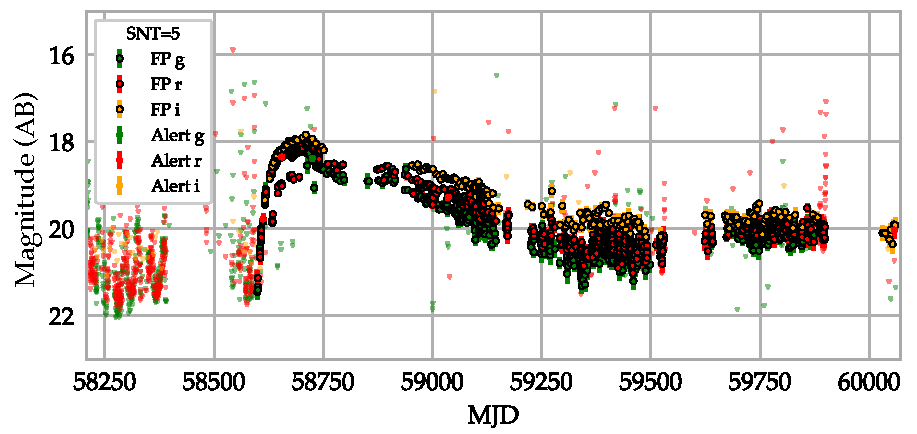
\includegraphics[width=1\textwidth]{at2019fdr/at2019fdr_lc_rebrightening.pdf}
    \caption[\emph{AT2019fdr} rebrightening]{\emph{AT2019fdr} late stage rebrightening. Starting around MJD $=59500$, the flux in all ZTF bands increased, until it reached a plateau $\sim 200$ days later.}
    \labfig{at2019fdr_rebrightening}
\end{figure}

After the publication of our paper on \emph{AT2019fdr}, the transient underwent significant rebrightening in the optical. About 2.2 years after the optical peak and a continuous decline ever since, the flux in all three ZTF bands started to increase again, until it hit a plateau roughly 200 days later. As of April 2023, \emph{AT2019fdr} is still in this plateau. This is atypical behavior for TDEs and SNe, as was already pointed out in~\cite{Frederick2021}. For now, it remains to be seen how long-lived that rebrightening is.

Interestingly, also \emph{PS1--10adi} showed late-stage rebrightening~\cite{Jiang2019}. For this transient, the authors discussed a variety of possible causes for that behavior. They concluded that late-stage accretion was unlikely, based on the different properties of the dust echoes of the initial flare and the rebrightening. They also discarded interaction between the debris and the SMBH torus, based on the fact that the complete conversion of the unbound debris' orbital energy was insufficient to explain the luminosity of the rebrightening. Instead, they favored a scenario where a mildly relativistic outflow from the TDE is responsible for the rebrightening~\cite{Jiang2019}.

It remains an open question if the long-lasting rebrightening of \emph{AT2019fdr} can be explained by such an outflow. One could also hypothesize that a perturbation in the accretion disk, triggered by the TDE, is responsible for the increased optical flux; see e.g.~\sidecite{Ricci2022}.

\subsection{Soft X-ray Signal and Dust Echo: More Evidence for a TDE}
As already discussed in Section~\ref{x_ray_obs}, an X-ray signal from \textit{AT2019fdr} was detected by \textit{SRG}/eROSITA on its third visit with an unusually soft thermal spectrum of \SI[parse-numbers = false]{56^{+32}_{-26}}{\eV}. As AGN X-ray spectra are rarely soft~\sidecite{Saxton2020}, this significantly strengthens the TDE interpration.

NLSy1 galaxies in general exhibit softer spectra, but the temperature of \emph{AT2019fdr} was atypically low also in this context: For example, it was lower than all NLSy1 temperatures in~\sidecite{Leighly1999} and~\sidecite{Vaughan1999}. Additionally, SLSNe rarely emit X-ray radiation. Only the first SLSN ever detected, \textit{SCP 06F6}~\sidecite{Barbary2008}, possibly showed an X-ray flux exceeding \emph{AT2019fdr}'s luminosity~\sidecite{Gaensicke2009}.

The dust echo (see Section~\ref{dust_echo}) we found, together with the energy budget and the bolometric evolution suggests that \emph{AT2019fdr} belongs to an emerging class of strong TDE candidates located in AGN, as e.g.\ \emph{PS1-10adi} (discussed above), \emph{AT2017gbl}~\sidecite{Kool2020}, or \emph{Arp 299-B AT1}~\sidecite{Mattila2018}.

\section{Chance Coincidence}
To compute the chance coincidence of observing a TDE comparable to \emph{AT2019fdr} in spatial and temporal coincidence with a high-energy neutrino in addition to the first neutrino-TDE association, I created a sample of TDEs and candidate TDEs of similar or higher brightness.

The sample from which these sources were selected was the full sample of nuclear transients as selected by a filter implemented in \texttt{AMPEL} (see Section~\ref{ampel}). This filter required at least 10 detections in both the \textit{g}- and the \textit{r}-band. Additionally, we required a weighted maximum distance of the flare to its host of $\leq \SI{0.5}{\arcsec}$, and that most datapoints had positive flux after subtraction of the reference image. A detailed discussion of the nuclear filter can be found in Section~\ref{nuclear_filter}.

I restricted the dataset to transients first detected after January 1, 2018 to ensure that all of them had high-quality reference images. I also required the transients to have peaked before July 2020. In total, 3172 flare candidates remained after these cuts.

I further required that the transients were not classified as variable stars, or bogus objects. Additionally, their rise (fade) $e$-folding time was required to exceed the uncertainty on this parameter. At this stage, 1628 candidates remained.

As only candidates with brightness comparable to or higher than \emph{AT2019fdr} were of interest, I required their peak apparent magnitude to be $\leq$ \emph{AT2019fdr}'s peak apparent magnitude; this left 157 transients. To select candidate TDE and accretion flares, I required the rise (fade) $e$-folding time to lie in a [15,80] ([30,500]) day interval, which left 25 transients.

Lastly, I excluded those transients from the sample of 25 transients which were spectroscopically classified as supernovae, or could be ruled out as short-timescale AGN variability by visual inspection. I also excluded candidates which displayed no consistent color or color evolution post peak, or which had a non-smooth light curve evolution post peak. This left a final sample of 12 transients.

I then calculated the effective source density $\rho_\text{eff}$---i.e.\ the density of sources per \unit{\square\deg} of sky in the survey footprint at any given time---as follows:

\begin{equation}
    \rho_\text{eff} = (N_\text{flare} \times \Delta t_\text{flare}) / (A_\text{ZTF}  \times \Delta t_\text{search}),
\end{equation}
where $N_\text{flare}$ is the total number of comparable sources (including \emph{AT2019dsg} and \emph{AT2019fdr}), $\Delta t_\text{flare}$ is the typical duration of such events, $A_\text{ZTF}$ is the sky area accessible to ZTF, excluding sources with a galactic latitude $|b|<\SI{7}{\degree}$, and $\Delta t_\text{search}$ is the time range of the sources sample, i.e.\ 2.5 years. With the 12 events of the comparison sample, the effective source density was $\rho_\text{eff} = \SI{1.71e-4}{\deg}^{-2}$.

Now an expectation value for the number of neutrinos coincident with two sources (\textit{AT2019dsg} and \textit{AT2019fdr}) can be calculated as $\mu=\rho_\text{eff}\times A_\text{IC}$, where $A_\text{IC}$ is the summed \SI{90}{\percent} uncertainty area of the alert neutrinos we followed up. This was \SI{154.33}{\square\deg} at that time, which resulted in $\mu=0.026$. Employing a Poisson distribution, the probability of finding two sources by chance was $p(2)=\num{3.4e-4}$, while finding one source only had a p-value of $p(1)=\num{2.6e-2}$~\cite{Reusch2022}.

To obtain the probability of finding two neutrinos coincident by chance, I calculated the probability of observing 0 and 1 coincidences, and subtracted these from 1---this yields the probability of observing two or more coincidences:

\begin{equation}
    p(2) = 1 - \sum_{k=0}^1 \frac{e^{-\mu}\mu^k}{k!},
\end{equation}
where the sum is the cumulative distribution function of the Poisson distribution. Using a right-tailed normal distribution, $p(2)=\num{3.4e-4}$ translates to $\SI{3.4}{\sigma}$ (\SI{1.94}{\sigma} for a single association).


\section{Dust-Echo TDEs as Neutrino Sources?}\label{at2019aalc}
I have so far detailed the data reduction for \emph{AT2019fdr}, established that it likely was a TDE---albeit an unusual one---modeled its SED and the dust echo we discovered, calculated its energy output and showed that a chance coincidence of two high-energy neutrinos with sources comparable to \emph{AT2019fdr} is quite improbable.

\subsection{Adding a Third Event: \textit{AT2019aalc}}
During the work on \textit{AT2019fdr}, another candidate emerged as a potential high-energy neutrino counterpart, also accompanied by a dust echo. This section is dedicated to that event, \textit{AT2019aalc}.

As both high-energy neutrino associated TDEs had prominent dust echoes, this prompted a search for other optical flares accompanied by a strong dust echo and in coincidence with high-energy neutrinos~\cite{Velzen2021}. That study found a third candidate counterpart that so far was missed as its sky location was inaccessible to ZTF at the time of neutrino detection due to its proximity to the sun.

\subsection{Event Details}
\textit{AT2019aalc} is the possible counterpart to neutrino \textit{IC191119A}~\cite{Velzen2021}. It featured the largest dust echo luminosity of all three transients, while the dust echo strength as defined in~\cite{Velzen2021} was a bit lower due to pre-flare variability.

In contrast to \textit{AT2019dsg} and \textit{AT2019fdr}, much less is known about \textit{AT2019aalc}. Early scanning discarded it as probable AGN activity (which it still could be), and it was not studied further until it emerged as neutrino counterpart candidate many months later (the neutrino itself arrived about 5 months after optical peak). For this reason, no UV measurements or spectra were taken. This is why the classification as a TDE is a much more tentative one, but nevertheless compatible with the light curve.

\textit{AT2019aalc}'s peak \textit{g}-band luminosity was comparable to \textit{AT2019fdr} and it was also detected by \textit{SRG}/eROSITA during one visit. Like \textit{AT2019fdr} and \textit{AT2019dsg}, it displayed a soft thermal spectrum with a blackbody temperature of $172^{+10}_{-10}$ eV; this counts as evidence favoring a TDE interpretation. Also, there was an archival radio detection by VLASS.

The chance coincidence of finding three such dust-echo events in spatial and temporal coincidence with a high-energy neutrino was found to be $3.7\sigma$. The soft X-ray detections were not part of the initial selection criteria, but rather emerged ex post.

\pagebreak

\subsection{Comparing the Candidate Counterparts}
Table~\ref{tab:comparison} shows a comparison of the relevant measurements and inferred quantities of the three events. One commonality is that the neutrino was significantly delayed with respect to the optical peak, by about 5--10 months. All transients were detected in X-ray wavelengths with a low temperature, and all were accompanied by a prominent dust echo. There have been attempts to draw conclusions from these facts.

\begin{table*}[htb]
    \centering
    \setlength{\tabcolsep}{12pt}
    \begin{tabular}{l  c  c  c}
        \hline
        \textbf{Property}          & \textbf{\textit{AT2019dsg}} & \textbf{\textit{AT2019fdr}} & \textbf{\textit{AT2019aalc}} \\
        \hline
        \hline
        TDE                        & yes                         & strong candidate            & candidate                    \\
        Peak bol. luminosity       & \SI{3.5e44}{\erg\per\s}     & \SI{1.3e45}{\erg\per\s}     & ---                          \\
        SMBH Mass                  & $10^{6}-10^{6.7} M_\odot$   & $10^{7.55} M_\odot$         & $10^{7.2} M_\odot$           \\
        Radio                      & evolving                    & not evolving                & archival det.                \\
        UV                         & very bright                 & bright                      & ---                          \\
        X-ray                      & early, soft spectrum        & late, soft spectrum         & soft spectrum                \\
        Dust echo strength         & $92.2$                      & $39.2$                      & $15.7$                       \\
        $\nu$ delay                & $\sim 5$ months             & $\sim 10$ months            & $\sim5$ months               \\
        $\nu$ production           & possible                    & possible                    & possible                     \\
        $\nu$ energy               & \SI{217}{\tera\eV}          & \SI{82}{\tera\eV}           & \SI{176}{\tera\eV}           \\
        $\nu$ 90\% uncertainty box & \SI{25.5}{\square\deg}      & \SI{25.2}{\square\deg}      & \SI{61.2}{\square\deg}       \\
        $\nu$ signalness           & 0.59                        & 0.59                        & 0.45                         \\
        \hline
    \end{tabular}
    \caption[Comparison of all counterpart candidates]{Comparing the multi-messenger properties of the candidate TDEs coincident with high-energy neutrinos. The dust echo strength was defined as $\Delta F/F_{\text{RMS}}$ (flux increase after optical/UV peak vs.~the root mean square of the pre-flare flux); `$\nu$ production' means that models exist showing that the source might be capable of producing a neutrino with the respective detected energy; for `$\nu$ signalness' see Definition~\ref{signalness_def}. `---' denotes insufficient modeling or missing data. Table by the author, adapted from~\cite{Reusch2023d}.}
    \label{tab:comparison}
\end{table*}

\begin{figure*}[htb]
    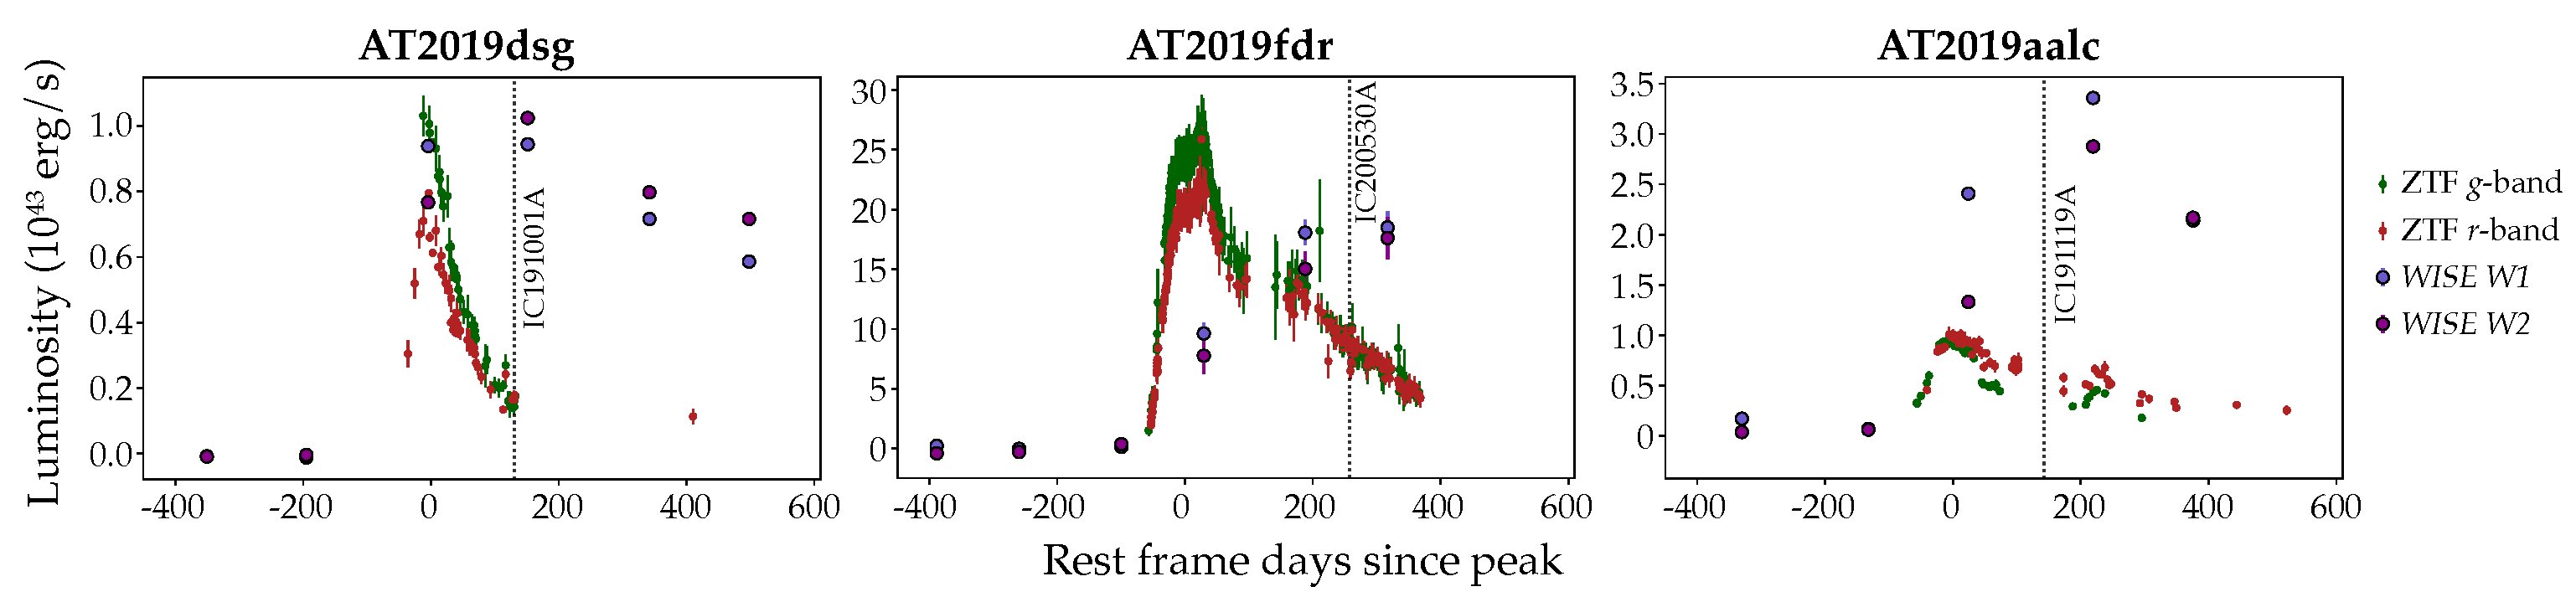
\includegraphics[]{AT2019fdr/comparison.pdf}
    \caption[All candidate counterparts in comparison]{All three candidate counterpart TDEs with ZTF optical light curve and \textit{WISE} detections, showing the relative strength of the dust echo. The neutrino arrival times are shown as black dotted vertical lines. Figure adapted from~\cite{Velzen2021}.}
    \labfig{dust_echo_comparison}
\end{figure*}

The observed delay might either be a statistical effect, or it could carry physical meaning. In~\cite{Velzen2021} it was explained by the assumption that the debris first has to circularize before the first neutrinos can be produced. In~\sidecite{Winter2023} the observed time delay of the neutrino was combined with the fact that the dust echo was peaking around the neutrino detection time for all three transients, as one can see in Figure~\ref{fig:dust_echo_comparison}.

One of the models presented in~\cite{Winter2023} makes use of that fact, as the photons from the dust echo serve as targets for the protons accelerated within the source. Therefore, the neutrino delay arises naturally from the delay of the infrared emission. The energies involved in this model would make TDEs interesting candidates for the production of Ultra-High Energy Cosmic Rays (UHECR). The downside of this model is that it requires very high proton energies.

A companion model swaps the infrared target photons for X-ray photons, as all three sources showed signs of soft X-ray emission. That model can also explain the time delay, which arises from the confinment of moderate energy protons in this case. The observed neutrino energies are explained better here, but the observed neutrino delay is described less well in comparison to the IR model. Lastly, a third model uses optical/UV target photons (as was done in~\cite{Velzen2021}). This yields the highest neutrino production efficiency, but does not explain the observed time delay of the neutrino.